
%
% Simple Latex 2e template
%
\documentclass[12pt]{article}
%\usepackage[usenames,dvips]{pstcol}q
\usepackage{color}
\usepackage{amssymb}
%\usepackage{epsfig}
\usepackage{footnote}
\usepackage{longtable}
\usepackage{verbatim}
\usepackage{array,multirow}
\usepackage{titlesec}
%
% You can't use subfigure and subcaption at the same time (!)
%\usepackage{subfigure}
%\usepackage{subfigure}
% new for subfigures
\usepackage{graphicx}
\usepackage{caption}
\usepackage{subcaption}
%\usepackage{subfigure}
%
% Using .ps files with pdflatex
%\usepackage{epstopdf}
% Instructions- do \includegraphics{file.eps} and then run pdflatex
%
%\usepackage{slidesec}

%\input{seminar.bug}
%\slidesmag{3}
%\usepackage[letterpaper]{geometry}
%\usepackage{fancybox}
%\usepackage{charter}
%\usepackage{feynmf}
%\usepackage{fancyhdr}
%\usepackage{pdfpages} % then do \includepdf{cv.pdf} to include the file cv.pdf
%
% make \paragraph a subsubsubsection
\setcounter{secnumdepth}{4}
%\titleformat{\paragraph}
%{\normalfont\normalsize\bfseries}{\theparagraph}{1em}{}
%\titlespacing*{\paragraph} {0pt}{3.25ex plus 1ex minus .2ex}{1.5ex plus .2ex}
%
%\include{symbols}
%
\textwidth 6.5in \textheight 9.5in \topmargin -0.6in \oddsidemargin
0.0in \evensidemargin 0.0in
\parindent 0.5in
\def\baselinestretch{1.0}
%
\def\changemargin#1#2{\list{}{\rightmargin#2\leftmargin#1}\item[]}
\let\endchangemargin=\endlist
%
%
\newcommand{\smaller}{\fontsize{8}{12}\selectfont}
%\newrgbcolor{maroon}{.45 0.1 0.1}
%
% Try making it behave with figures
%
\renewcommand{\topfraction}{0.85}
\renewcommand{\textfraction}{0.1}
\renewcommand{\floatpagefraction}{0.75}
% \enlargethispage*{240.1in} To over-ride the float dogmas- follow by \newpage
%
%
\def\LAPPDTM{LAPPD\textsuperscript{TM}~}
\def\LAPPDTMs{LAPPD\textsuperscript{TM}s~}
\def\LAPPD{LAPPD~}
\def\LAPPDs{LAPPDs~}
\def\FTBF{Fermilab Testbeam Facility~}
\def\eightbyeight{$8'' \times 8''~$}
\def\MTEST {\textsc{MTEST}}
\def\OTPC {Optical Time Projection Chamber}
\def\TPC {Time Projection Chamber}
\def\TOF {Time of Flight}
\def\QE {Quantum Efficiency}
\def\micron {$\mu$m}
\def\microns {$\mu$ms}
\def\epem{$e^{+} e_{-}$}
\def\sigT{$\sigma_T$}
\def \sigL {$\sigma_L$}
\def \ge {$\gamma e$}
\def \chisquared {$\chi ^2$}
\def \chisq {$\chi ^2$}
\def \F18 {$^{18}F$}
\def \gam {$\gamma~$}
\def \gams {$\gamma s~$}
%
%\def\PE {photoelectric_effect}
%
%
%
% Begin document
%

\begin{document}
\pagestyle{plain}
%\renewcommand{\headrulewidth}{0pt}
%
\begin{flushright}
%Version 1.0\\
\today
\end{flushright}

%
% Title
%
\begin{center}
{\Large\bf A TOPAS Simulation of High-resolution Low-Z-Medium Whole-Body TOF-PET}\\
\vskip 0.3in
%{\Large\bf DRAFT}

Kepler Domurat-Sousa, Cameron Poe, Jo\~ao F. Shida, Eric Spieglan, Evelyn Sun, Bernhard W.
Adams, Evan Angelico  Henry J. Frisch, Patrick La Riviere, Allison
Squires

{\it to be submitted to Medical Physics: The International Journal of
Medical Physics Research and Practice}
\end{center}

\vskip 0.5in

\begin{abstract}
%{\bf\Large Abstract}\\
We have used the TOPAS Geant4-based simulation package to simulate a
TOF-PET system employing a low atomic number liquid medium such as a photoswitchable
organic scintillator rather than the conventional high-Z crystals.
In a low atomic number medium the Compton scattering of a
gamma from the positron annihilation dominates the absorption via the
photo-electric effect, resulting in a chain of scatterings at
successively lower gamma energies, each producing a recoil Compton
electron that deposits ionization energy along its track. Multiple scattering
and rate of ionization ($dE/dx$) depend on electron velocity and so can be
used to identify the start of the recoil electron track at one end-point
of the Line-of-Response (LOR).

The TOPAS package was used to simulate a cylindrical detector consisting of xx-cm thick
xxx surrounding a bore diameter of xxx cm and covering the range in polar angle $-xxx^o - xxx^o$, filled with
linear alkylbenzene (LAB) liquid scintillator as the ionization medium.
Optical high resolution reconstruction remains to be developed; one example being
explored is a low concentration (e.g. $10^{-xxx}$) of a (hypothetical) photoswitchable dye. %needs rewriting
The LOR in each event was reconstructed
via a time-ordering of the energy deposited by the successive Compton
electrons.

Simulations have been performed for the Derenzo phantom and XCAT
brain and lung phantoms to determine event reconstruction
efficiencies, transverse resolutions, and image signal-to-noise.
Mis-reconstructed events have a lower contrast than events with both
ends of the LOR correctly identified by several orders-of-magnitude,
forming a smooth background that is subtracted via a maximum
likelihood fit to an expansion in Zernike functions.
Locating the annihilation longitudinally on the LOR
is implemented by large-area fast time-of-flight photodetectors with
single photon time resolution in the tens of ps and sub-mm spatial
resolution. In-patient scattering is rejected with efficiencies of xxx
and xxx for the XCAT brain and lung phantoms, respectively. The
simulations indicate a possible large reduction of dose. The
development of suitable photoswitchable dyes or other image-persistent
economical low-Z media may be possible.
\end{abstract}
%\end{center}

\newpage
\tableofcontents

\listoffigures

\listoftables

\newpage
\section{Introduction}


%Low Z, Compton-chain, resolution, large-area psec TOF, dose reduction,
%applications

% Advances beyond the first paper- full detector simulation rather than just the gamma, in-patient scattering, mis-identification, efficiencies, post-simulation analysis

Precision Time-of-Flight Positron-Emission Tomography (TOF-PET) has
become immensely
sophisticated~\cite{Vandenberghe_Moskal_Karp_review_2020,Vaquero_Kinehan_review_2015,Phelps_Cherry_Dahlbom_book_2006}.
Among other innovations, state-of-the-art whole-body scanners have been
built and
characterized~\cite{Vandenberghe_Moskal_Karp_2020_Whole_Body_PET_2020,Cherry_Explorer_scattering_2019},
TOF-PET with sub-nanosecond coincidence~\cite{Lee_Levin_100ps_2021} has
recently been developed, an international competition to develop sub-10
ps TOF resolution~\cite{lecoq_2019} is now in place, and timing with
resolutions of 10 psec or below using MCP-PMT photodetectors and
Cherenkov light in
pre-radiators~\cite{Credo,Ohshima,Anatoly_TestBeam_2010} is being
developed by Cherry et al. for higher spatial resolutions and lower
doses~\cite{Cherry_Hamamatsu_2021}.

A worthy goal for further TOF-PET development is to achieve resolutions
set by the underlying physics processes rather than the detector
segmentation~\cite{Moses_Fundamental_Limits}. In this context, we have
been exploring PET scanners based on the development of fast large-area
(400 cm$^2$) MCP-PMT-based
photodetectors~\cite{history_paper,timing_paper,Limitations_Workshop_2011,Andrey_paper_1}
 with low-cost high-speed waveform sampling data-acquisition~\cite{PSEC4, OTPC_paper}
viewing low atomic number scintillating
media~\cite{Moskal_Organic_Scint_2012,PET_NIM_paper,PET_patent}.


In a low atomic number scintillation medium such as an organic
scintillator~\cite{Kamland-Zen}, the Compton scattering of a 511 keV
gamma dominates absorption via the photo-electric effect by a factor of
$~10,000$~\cite{cross_sections}, resulting in a chain of scatterings at
successively lower gamma energies, each producing the track of a recoil
electron in the detector medium. Measurement of the locations of the
scatters, the relative angles between successive scatters, the plane of
the scattering, and the deposited energies and directions of the recoil
electrons allows using the kinematical constraints of the 2-body
Compton scattering process to perform a statistical time-ordering of
the gamma interactions.

Initial studies showed that
reconstructing the recoil electron tracks may enable a time-ordering of
the Compton scatterings in the detector, with a high probability of
precisely identifying the site of the first interaction of each
gamma~\cite{PET_NIM_paper}. Connecting the locations of the first
interaction for both gammas provides the determination of the
line-of-response (LOR) with a transverse resolution determined by the
underlying physical processes. Additionally, large-area MCP-PMT-based
photodetectors can provide cm-scale TOF resolution along the
LOR~\cite{PET_NIM_paper}. The TOF system also measures the time and
location of individual photons from the successive Compton scatterings
and consequently allows disambiguation of multiple events. Optimizing
images from the complex ensemble of locations, scattering planes,
times, and energies in each event will require advanced analysis
techniques beyond the scope of this work.

 The scattering angles of the gamma and the energy of the scattered electron are determined by conservation of energy and momentum in the 2-body Compton process, providing handles on reconstructing the correct time-ordering. The earlier (higher energy) end of an electron track can be statistically determined from energy deposition and angular scattering. There are additional constraints from the requirement that the LOR connecting the 2 first-scatters must lie in the plane of the scattering determined by the angles and the electron track, and the angle between the two planes has a dependence predicted by the quantum entanglement of the two gamma polarizations. The TOF system may provide additional information constraining the time-ordering of the creation of the electrons.

There are candidate low-Z media that retain the imprint of local
ionization  through different persistence mechanisms, including those
with a change in molecular states, and others in which the change is
thermodynamic, as in a bubble chamber~\cite{glazer_bubble_chamber}. For
a specific example, we have previously discussed the potential for
development of appropriate two-state photoswitchable organic
dyes~\cite{PET_NIM_paper}. In these cases energy resolutions on the
order of a few percent or less may be achievable~\cite{PET_NIM_paper}.

 In this present paper we present simulations using the TOPAS
 Geant4-based framework~\cite{TOPAS} of a TOPAS-generated whole-body TOF-PET detector similar to
that of Ref~\cite{PET_NIM_paper}. TOPAS is much more user-friendly and
transparent than the raw Geant4 used in our previous work. Topas also
provides access for the user to add physics and analysis, as well as
the opportunity to add code to extend and check the underlying physics.
TOPAS also provides excellent user support.

 The organization of the paper is as
follows; Section~\ref{TOPAS} provides an introduction to TOPAS and
describes the modifications for the whole-body TOF-PET analysis.
Simulation results for the Derenzo phantom and an ideal detector are
reported in Section~\ref{Simulation}. The analysis and results on TOF
resolution are described in Section~\ref{TOF}. Rejection of in-patient
scattering through timing, gamma energy reconstruction, and the
coplanarity and scattering plane correlations intrinsic in the 2-gamma
emission from positron annihilation are presented in
Section~\ref{In-patient_Scattering}. The reconstruction of the LOR, including
inefficiencies due to mis-reconstructions and geometric
acceptance, are discussed in Section~\ref{Reconstruction}.
Section~\ref{Imaging_phantoms} presents images and figures-of-merit for imaging
the Derenzo phantom and the  XCAT phantom of Alan
Dershowitz~\cite{Dershowitz_phantom}. A brief summary is given in
Section~\ref{Summary}.

%\vspace*{-1.5in}
\begin{figure}[!ht]
	\centering
	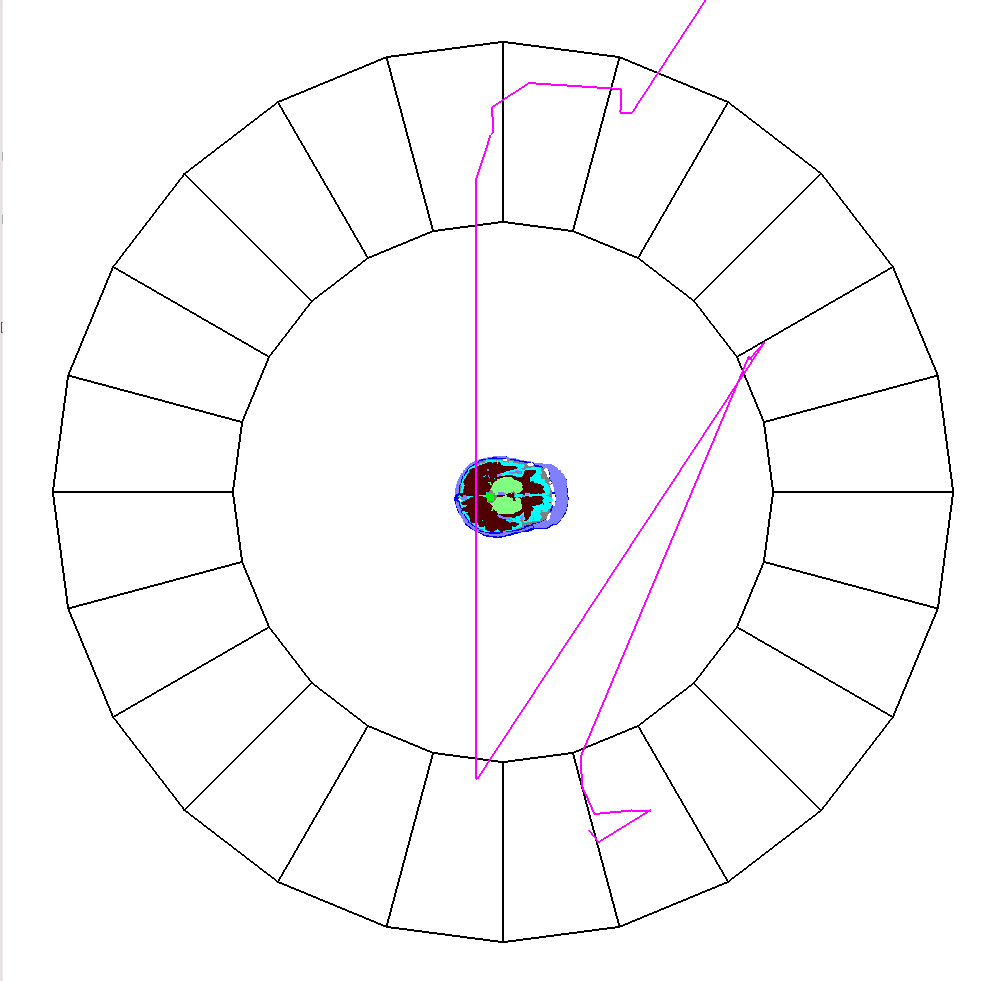
\includegraphics[angle=0,width=0.37\textwidth]{Figures/brain-gammas-figure-inverted-v1a.png}
	\caption{A TOPAS representation of a TOF-PET detector with a
	  superposed simulated annihilation event in the patient.}
	\label{fig:Detector_and_Gamma}
\end{figure}

\begin{figure}[ht]
	\centering
	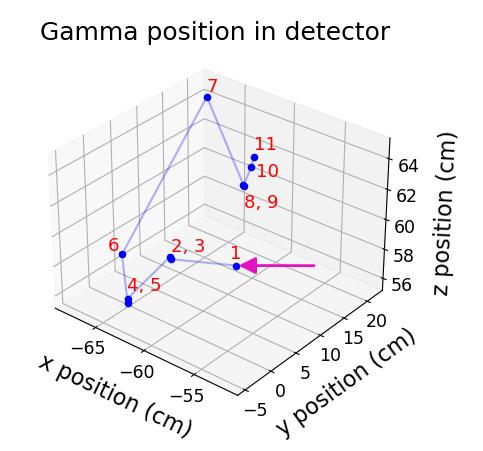
\includegraphics[angle=0,width=0.28\textwidth]{Figures/gamma-scatter-figure-v1a.png}
	\caption{The simulated electron tracks in a detector module corresponding to
 the chain of successive gamma-e Compton scatterings initiated by a
 511 keV gamma from the \epem annihilation in the patient.}
	\label{fig:Detector_Module}
\end{figure}

\begin{figure}[ht]
	\centering
	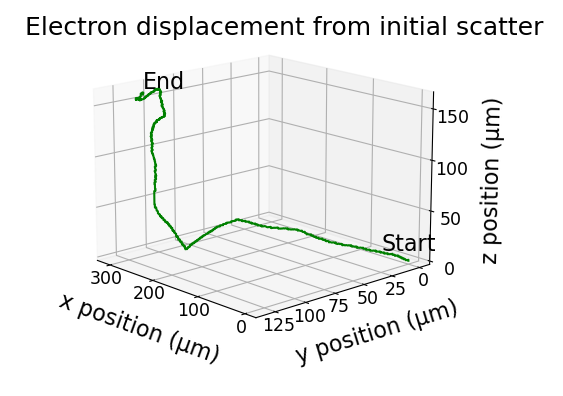
\includegraphics[angle=0,width=0.28\textwidth]{Figures/electron-scatter-figure-v1a.png}
	\caption{The path of the electron from a high energy scattering event. Using the increasingly twisty path of the electron as it has lower energy the origin of the electron can be determined.}
	\label{fig:Electron_Path}
\end{figure}

\section{The TOPAS Geant4-based Simulation Framework}
\label{TOPAS}
(Kepler's section- suggested paragraphs one per line below)

Introduction to TOPAS w references;\\
Goals and guiding principles of the simulation implementation;\\
Modifications and compromises (e.g. simplified detector,... ) for the results presented here.\\

TOPAS is a medical physics wrapper for Geant4. It allows for configuring Geant4 using text parameter files defining geometry, materials, particle sources and particle behavior recording. \\
TOPAS has allowed us to build a full simulation of a PET scanner with changeable phantoms. \\
Using a custom TOPAS scorer it was possible to get full data on particle interactions, allowing for the creation of a full simulation of event reconstruction. \\

\subsection{Functional description of the simulation}

The TOPAS simulation takes a description of a patient and detector and does all of the particle transport that results.\\
The result of the particle transport can then be input into reconstruction algorithms.

\subsubsection{Overview of flow}
The TOPAS simulation combines two parameter files: one defining the phantom and one defining the detector. \\
When run the simulation creates positrons within the phantom based on given activity data. \\
TOPAS uses Geant4 to do the particle transport simulation, including any Compton scattering that occurs in the patient or detector. \\
The desired data is then output in a file recording particle location, energy, and identifying information. This file is then used for the reconstruction algorithms. \\

\subsubsection{Input}
 (see Section~\ref{Detector})

The input is divided into two definitions: the detector definition and the phantom definition. Using TOPAS’s system for file inclusion these can easily be changed independently.\\
The detector file defines the shape and material of the detector, along with how events occurring in it will be recorded.\\
The phantom file defines the shape, material, and activity of the phantom.\\
A Derenzo phantom was created using cylinders with varying activities. // not really sure how valuable it is to say how I defined the Derenzo. It’s pretty obvious to anyone who has taken the TOPAS introduction course.\\
For a simulated patient the XCAT phantom was used. This is a 3d simulated patient with variation between tissues.\\



\subsubsection{Custom additions to TOPAS}
TOPAS allows for the creation of simulation aspects that are not a part of the software by default. In our case we needed information on particle location and energy within the detector.\\
The TOPAS extension framework allows direct contact with the underlying Geant4 for the specific cases where it is needed.\\
We created a custom tuple scorer for TOPAS that output particle energy, energy deposited in a step, position, and identifying information.\\
The custom scorer outputs the information for any geometry it is applied to. We typically made one file with particle data from the entire simulation, and a second only with information from inside the detector volume.\\


\subsubsection{Output data: energy, position, time, particle-type, particle index, parent process}

  Reference to DocLib note/UC websites etc. on formats ?

Using the flexibility of TOPAS and the custom scorer we were able to quickly get various data we desired from Geant4.\\

We measured the behavior of positrons in our simulation by tracking the start and end of each positrons history in the custom scorer. By subtracting the starting position from the ending position we got the positron displacement behavior. By checking the energy prior to annihilation we determined how often Geant4 was giving annihilation with substantial residual momentum in the detector frame.

\begin{figure}[!ht]
	\centering
	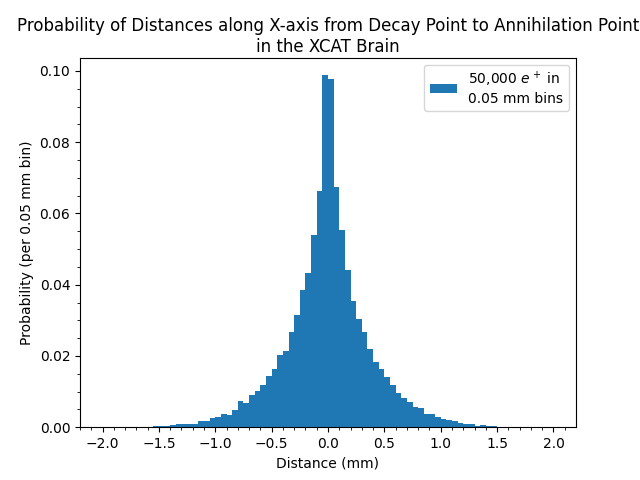
\includegraphics[width=0.45\textwidth]{Figures/xdist-v2.1.png}
	\hfil
	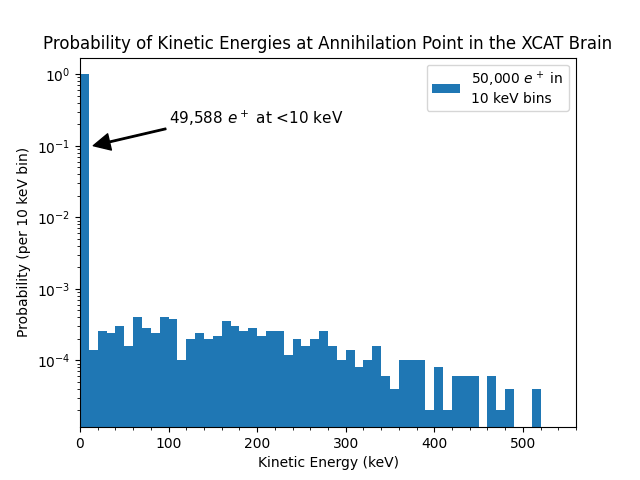
\includegraphics[width=0.45\textwidth]{Figures/finale_log-v2.1.png}
	\caption{Data from TOPAS showing the displacement and energy of positrons at annihilation. Both histograms are from runs with 50000 positrons. Left: The distance traveled along the x-axis by positrons from their creation to their annihilation. Right: A log plot of the energy at annihilation of the positrons. The vast majority of positrons annihilate with no residual energy. In the zero bin 49584 of 49588 events are identically zero energy.}
	\label{fig:positron_position_and_final_energy}
\end{figure}

\subsubsection{Custom additions- Cherenkov emission, positron scattering}

We used the following particle transport modules ``g4em-standard\_opt4'' and ``g4em-penelope''\\
TOPAS made the addition and removal of these packages the change of a single line of a parameter file. This allowed us to add the ``g4optical'' module to produce cherenkov light when measuring timing resolution in the modules.

%KEPLER IS HERE

\subsubsection{Limitations, approximations, missing processes}

\subsection{Post simulation processing}


TOF. Cluster finding; Advanced methods, including adaptive weighting, other?

\subsection{XCAT phantoms}
\label{XCAT_phantoms}
The 4D Extended Cardiac-Torso (XCAT) Phantom Version 2.0 is a software program that can simulate detailed patient anatomies for use in medical imaging. XCAT outputs binary files of voxelized male and female phantoms representative of a 50th percentile U.S. adult. Further anatomical variation and customization options are available. In addition, XCAT can simulate cardiac plaque, cardiac defects, and arbitrary spherical lesions~\cite{xcat_2010_paper}.

TOPAS can read ImageCube-formatted data to create voxelized geometry components. ImageCube-formatted data refers to any binary data that contains one value per voxel. For the case of XCAT, each value is a different XCAT material or tissue. TOPAS then allows the user to specify the density and atomic composition of each material in the phantom [cite topas site?].

Patient simulations in this paper use the male XCAT phantom with no anatomical variations from normal. For defining the materials in TOPAS, we used data for male adults from the Annals of the International Commission on Radiological Protection (ICRP) P89, P110, P145, and International Commission on Radiation Units and Measurements (ICRU) Report 46~\cite{icrp89, icrp110, icrp145, icru46}.

\section{Simulating a model low-Z whole-Body TOF-PET Detector}
\label{Simulation}

We have previously described a whole-body TOF-PET scanner based on a low-Z medium
containing a fast scintillator and a persistent medium such as a
Switchillator photofluor~\cite{PET_NIM_paper}. We described a technique of time-ordering the Compton scatterings to precisely locate each end of the LOR, and the use of fast large-area TOF in a detector module. Here we present simulation results for an example whole-body detector, taking into account in-patient scattering (IPS), misidentifications, and detector resolutions.

Subsections~\ref{Detector} and ~\ref{Scintillating_media} describe the model detector
and the scintillating media, respectively. Subsection~\ref{Compton_chain} describes determining
the time-ordering of the Compton scatters in the ideal case
by using the Compton kinematic constraints to find the
location of first scattering. Table~\ref{tab:selection_efficiencies}
presents the efficiencies for finding the the correct gamma interaction points, and hence the ends of the LOR at high resolution. Subsection~\ref{Sigma_T} presents the
extraction of the transverse resolution on the end-points.

An example of an implementation of the method beyond this parametric implementation is given in Appendix A, which presents the results of a voxelation of the detector volume and the reconstruction of the Compton recoil electron tracks by a shoulder-seed cluster-finding algorithm.

\subsection{Detector Geometry}
\label{Detector}

% Figure 1-- Detector End View plus event
%
An example low-Z whole-body PET scanner with a simulated annihilation event from TOPAS superimposed is shown in Figure~\ref{fig:Detector_and_Gamma}. The location of the annihilation is indicated by the star; the successive interactions in the detector by Compton scattering are indicated by the resulting electron tracks in the low-Z medium. The location of the first scatter of each gamma determines the corresponding end of the Line-of-Response, with the goal of a transverse resolution measured in tens of microns~\cite{PET_NIM_paper}. The superposition of many lines of response gives a point-spread function with the transverse resolution~\cite{PET_NIM_paper}.



\subsection{Scintillating Media}
\label{Scintillating_media}
The scintillation medium assumed here comprises an organic solvent, a fast scintillator for the initial coincidence that triggers the data acquisition sequence, a photo-switchable dye that records the ionization from tracks of the Compton recoil electrons for repeated interrogation, and possible sensitizers to transfer energy from the solvent to the photo-switchable dye. We have taken the properties of the Kamland-Zen scintillator~\cite{Kamland_Zen} for the simulation of the Compton chain.
For the TOF simulation, we have assumed the fast scintillator has a 2 ps risetime~\cite{Buck_private_comm} and a (single) decay time of xxx ps.

\subsection{Characteristics of the Compton Chain of Successive Scatters}
\label{Compton_chain}
At 511 keV, the Compton scattering cross-section dominates the
Photo-electric cross-section by a factor of $10^{4}$, resulting in a
chain of successive Compton scatterings, with each one producing an
ionizing electron and a gamma with lower energy. In the low-Z medium the
scatterings are typically separated by distances of cm, several orders-of-magnitude
larger than the intrinsic resolution. Figure~\ref{fig:distance_traveled} shows
the results of the TOPAS simulation on the distance traveled in the medium
to the next scattering by: 1) an incoming initial 511 keV gamma; 2) the gamma resulting from the first scattering;
and 3) the gamma resulting from the second scattering. The peaking of the distribution for the initial  gamma is
due to the energy dependence of the Compton scattering cross-section


%\vspace*{-1.5in}
\begin{figure}[!ht]
\centering
  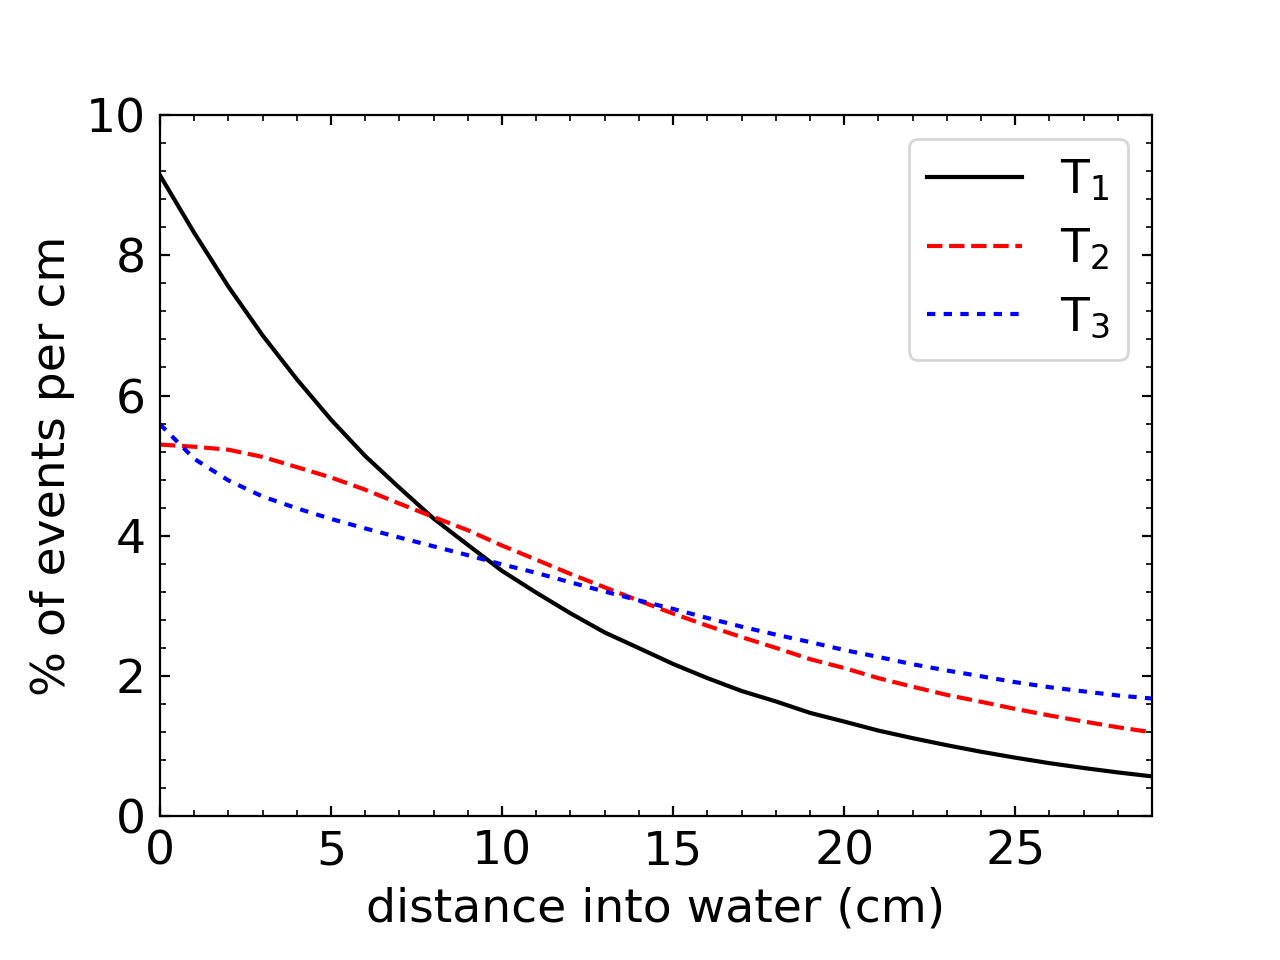
\includegraphics[width=0.45\linewidth]{Figures/scatter_dist_v1.png}
\caption{Distance in the detector medium traveled by: an initial 511 KeV gamma (black solid line);
the outgoing gamma from the first Compton scattering (red dashed line); and  the outgoing gamma from the 2nd Compton scattering (blue dotted line). T1 through T3 are the first through third true scatters.}
\label{fig:distance_traveled}
\end{figure}


\subsubsection{Compton scattering 2-body kinematics}
 The 2-body kinematics
of each scattering constrain the scattering angles and the outgoing
energies~\cite{PET_NIM_paper}. The goal is to use the constraints to
time-order the observed successive ionization sites to locate the first
scatter, with the start of that ionizing track being one end of the
LOR~\cite{PET_NIM_paper}.

Fig.~\ref{fig:angle_energy} shows the relationship between the gamma scattering
angle and the recoil electron energy due to the 2-body Compton
scattering kinematics for a 511 keV gamma.  The inset shows the profile at scattering angle of
$\theta=0.71$ radians.  The profile width is due to xxx.

\begin{figure}[!ht]
\centering
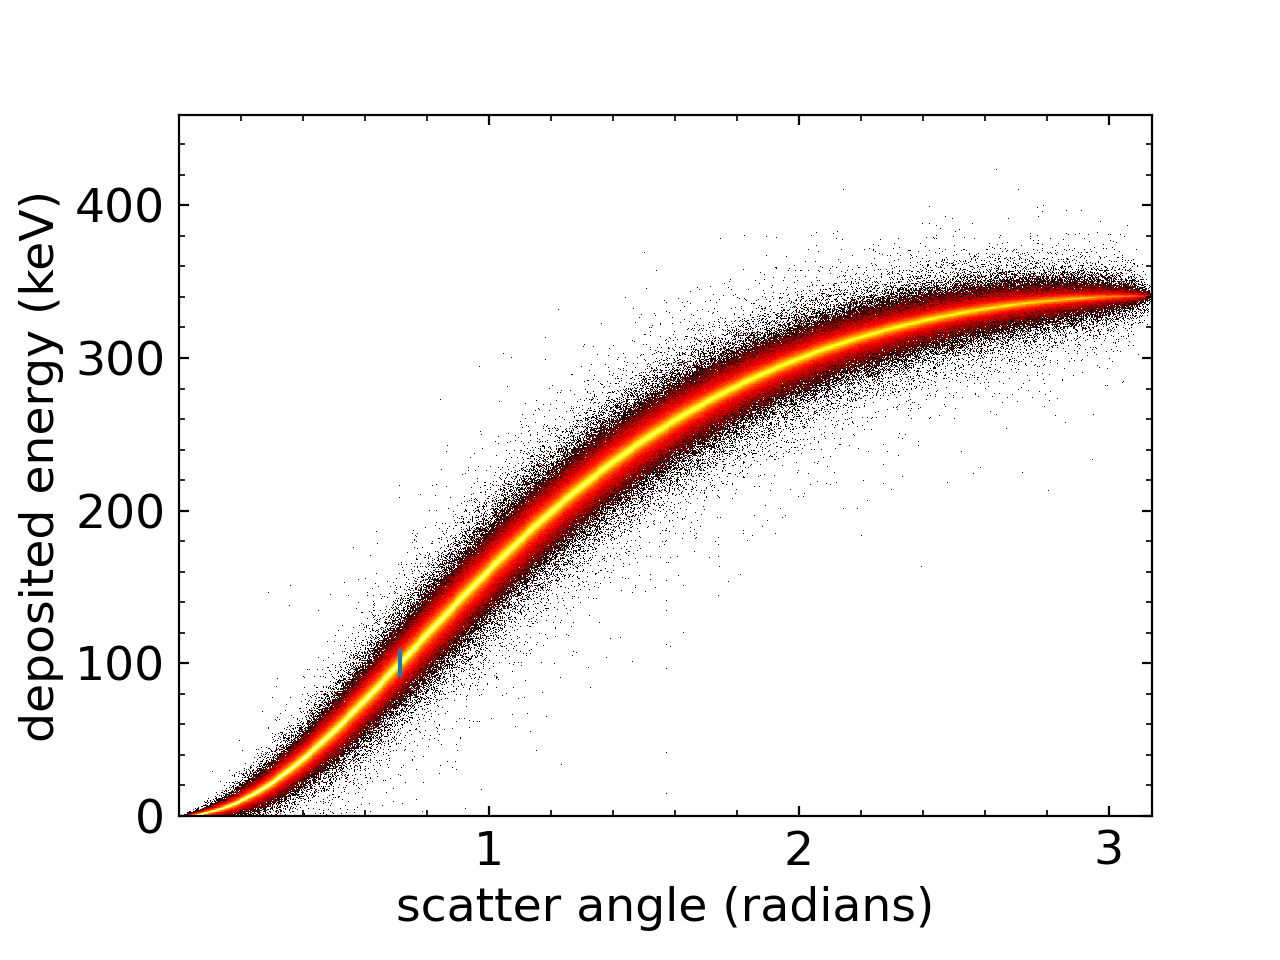
\includegraphics[width=0.45\textwidth]{Figures/compton_snake_v1.png}
\hfil
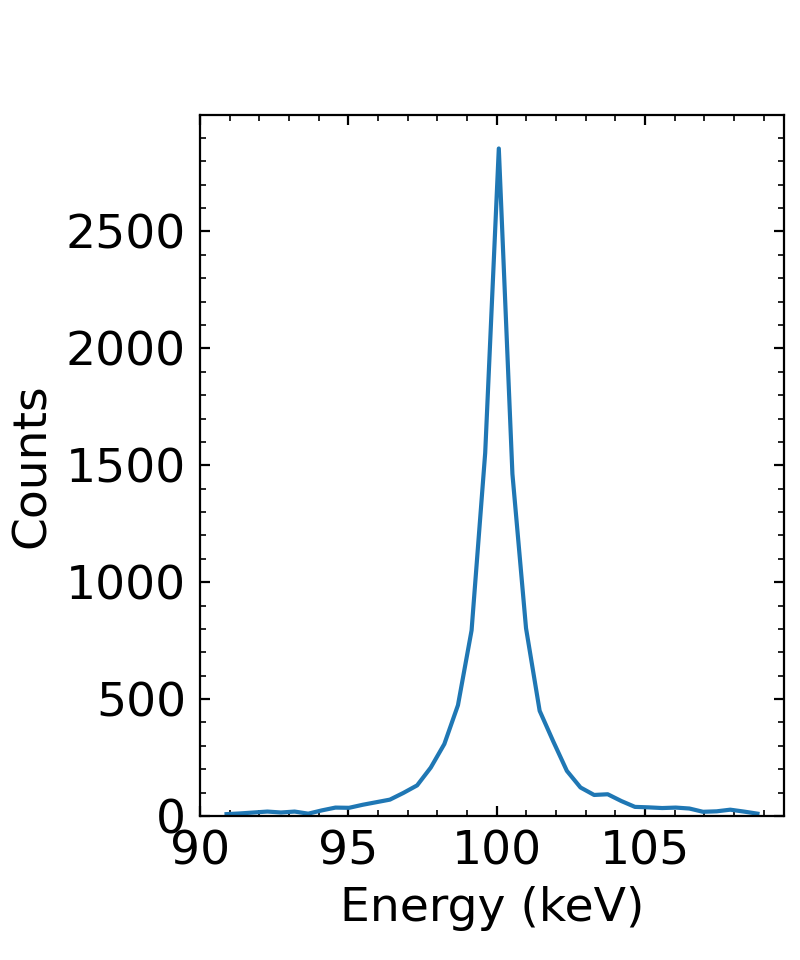
\includegraphics[width=0.28\textwidth]{Figures/compton_slice_v1.png}
\caption{The energy of the recoil electron versus the scattering angle for a 511 keV gamma as reconstructed by TOPAS, showing the kinematic constraint of 2-body scattering. The inset shows the profile at scattering angle of xxx$\theta=1.5$. xxxxxx The yellow line follows the theoretical prediction to within XXX}
\label{fig:angle_energy}
\end{figure}


\subsubsection{Reconstructing the chain of successive Compton scatterings from the TOPAS simulation}
We identify the order of the generated (true) scatterings by T followed by
numbering ($T_1,T_2,..T_i...$), while the ordering of the scatterings as reconstructed from
the analysis is labeled by R and numbering ($R_1,R_2,..R_i...$.
For example, in this notation a successful
reconstruction of an LOR end-point is when the $R_1$ reconstructed
cluster is the generated cluster with `scatter index' $T_1$.

Figure~\ref{fig:true_vs_reconstructed} plots the fraction of time (\%) the $T_i$th
recoil electron track is the cluster with the highest deposited energy,
i.e. the T$_1$-scatter (rhomboids), the T$_2$-scatter (squares),
the T$_3$-scatter (circles), and the T$_4$-cluster (pentagons). The first scatter is the cluster with
the highest energy for close to 60\% of scatter, and the set of the
$\mathrm{T}_1,\mathrm{T}_2,\mathrm{T}_3,\mathrm{T}_4$ energy depositions contains the first scatter in
xxx \% of gammas. Fig.~\ref{fig:2nd_plot} plots the distributions in
energy deposited by the recoil electron for scatter index $N_1$
(squares); $N_2$ (circles); $N_3$ (rhomboids).
%AAAAHHHHH update me!

%\vspace*{-1.5in}
\begin{figure}[!ht]
\centering
  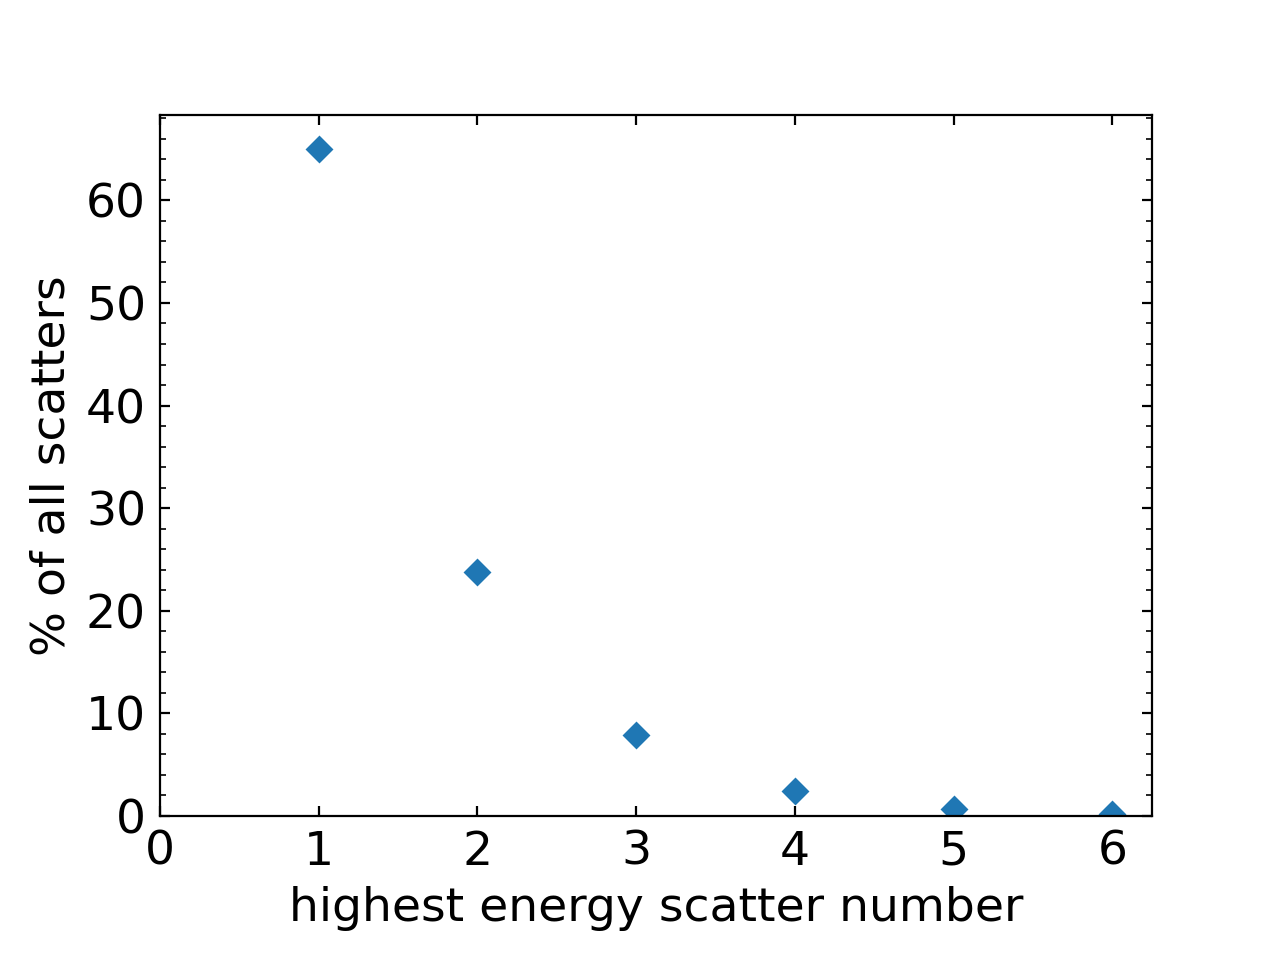
\includegraphics[width=0.45\textwidth]{Figures/scatter_with_highest_energy_v2.png}
  \hfil
  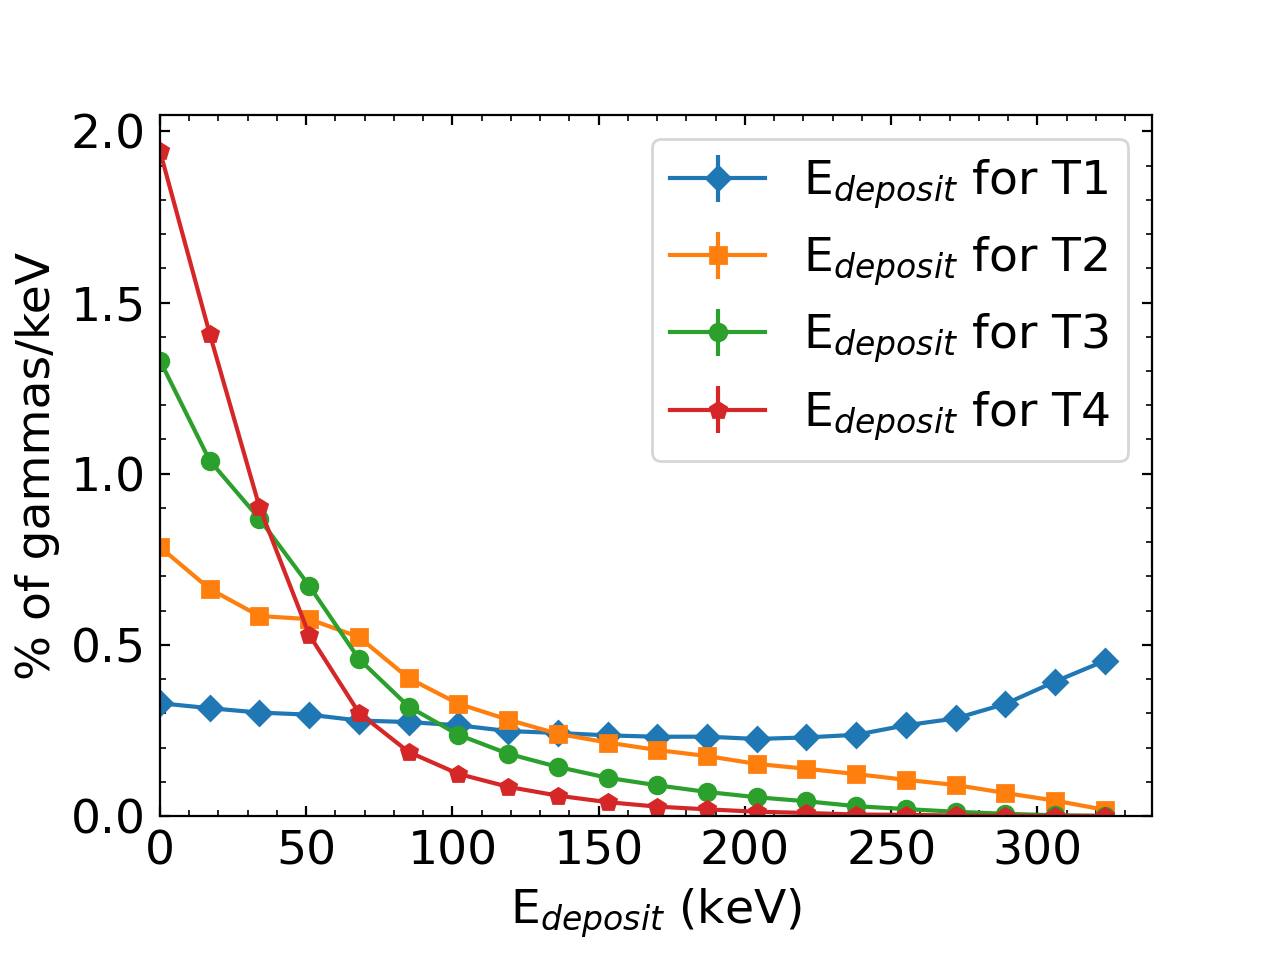
\includegraphics[width=0.45\textwidth]{Figures/T_eng_errorbar_v2.png}
\caption{Left: xxx The fraction of successive Compton scatterings that deposit the highest energy (are `brightest') of all scatterings.  Right: xxx The distribution in energy deposited for the first scattering (rhomboids); the second scattering (squares); the third scattering (circles), and the fourth scattering (pentagons).}
\label{fig:true_vs_reconstructed}
\end{figure}

\subsubsection{Containment and back-scattering}
The many-cm pathlength between Compton scatterings and the large angular range of the
outgoing gamma result in substantial inter-module scattering and escaped gamma due to
backscattering~\footnote{We note that back-scattering produces the highest energy electrons,
leading to good resolution on electron direction and starting point.}.
The number of scatters suffered by a gamma before escaping the module
is shown in the left-hand panel of Fig.~\ref{fig:escaping}. The energy deposited by a gamma
before escaping the module is shown in the right-hand panel for both all
scatters and for the T1 scatter.

\begin{figure}[hb!]
  \centering
  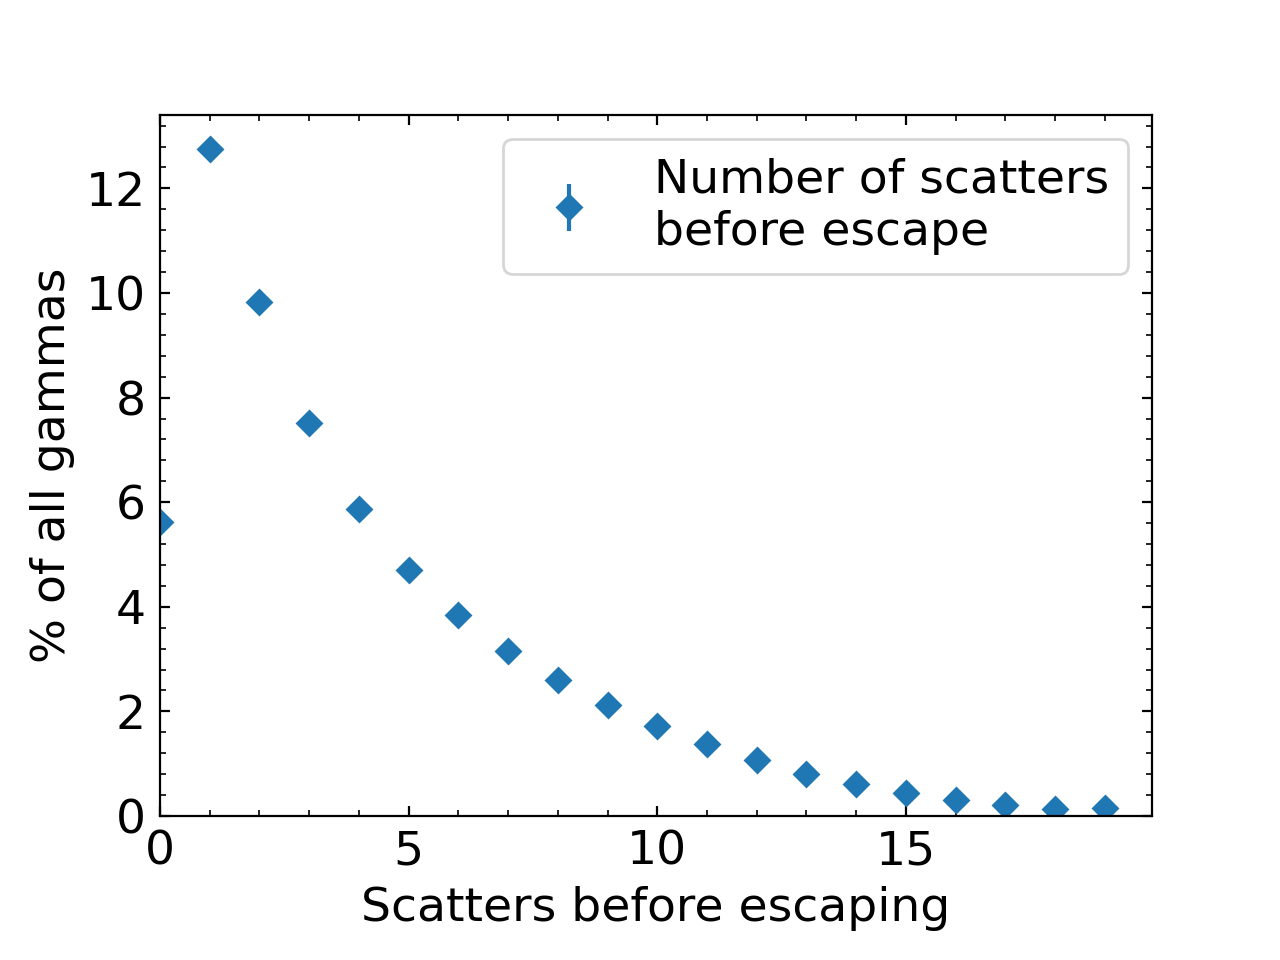
\includegraphics[width=0.45\textwidth]{Figures/scatters_before_escape_v3.png}
   \hfil
   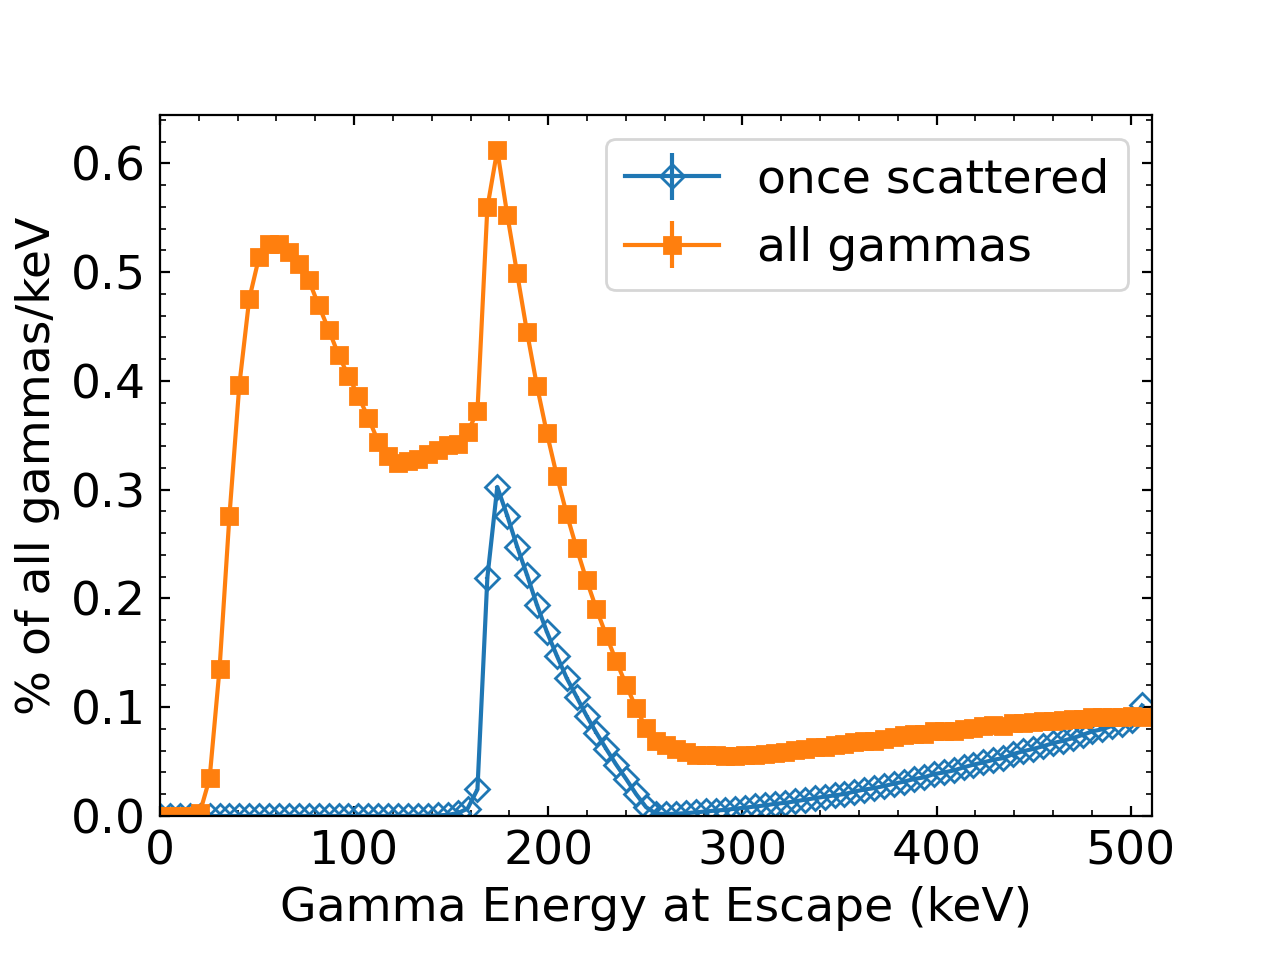
\includegraphics[width=0.45\textwidth]{Figures/energy_at_escape_v2.png}
\caption{An example simulation of containment for a 30cm deep module with water as the medium, and a gamma
entering at 45 degrees to the normal. Left: Number of scatters suffered by a gamma before escaping the module. Right: Energy deposited by a gamma before escaping the module for all scatters and the T$_1$ scatter. }
\label{fig:escaping}
\end{figure}
\clearpage

\section{Reconstructing the Line-of-Response}
\label{Reconstruction}
The TOPAS simulation allows us to estimate the reconstruction efficiencies, backgrounds, and resolution using a cut-based parametric analysis~\footnote{In contrast to the parametric analysis, an analysis based on a voxelized volume, simulated electron tracks, and a seed-shoulder based clustering algorithm is presented in Appendix A.}.

 \subsection{Finding the recoil electron track from the first scatter of the gamma}

Each end point of the LOR is found by cycling over the 10xxx highest-energy tracks in the triggering module and its neighbors, calculating a goodness-of-fit to the kinematic constraints for each combination. The figure of merit is
 \begin{equation}
\chi^2 = \Sigma etc.
\end{equation}
where the uncertainties in energy and angle are xxx and xxx, respectively.

\subsection{Finding the point of first scatter in the electron track}
\label{point_of_first_scatter}

For an as-yet unscattered gamma, the trajectory, and hence the LOR, ends at the start of the recoil electron track. The simulation accounts for multiple-scattering and energy loss along the electron track. We use the evolution of these two processes as the electron energy decreases along the track to determine which end of the track is the site of the gamma scattering. The figure of merit is:
\begin{equation}
\chi^2 = \Sigma Compton energy uncertainty formula %needs the full equation for uncertainty of Compton scattering (in the code)
\end{equation}
where the uncertainties in energy and angle are $\delta_E$ and $\delta_\theta$, respectively.

The scatters are used to form a tree of possible paths. If there are more than 10 scatters, the lowest energy scatters are ignored. All paths starting from the remaining scatters are tried. The search works by xxx a description of the tree behavior, including far side requirements. Possibly also include $\alpha,\beta$ pruning?

\subsection{Misidentified first scattering points}
A feature of the large disparity between the transverse resolution \sigT (10's of microns) and the scale of the separation between successive scatters (10's of cm) is that tracks misidentified as first scatters have LORs that miss by cm, and so form a low-frequency low-contrast background to the high-contrast correct orderings. This background is subtracted in the maximum likelihood fit to lower orders of a set of complete functions (see Section ~\ref{Zernicke_fits}).

\subsection{Reconstruction efficiencies for signal, in-patient scattering, and mis-reconstructed events}

Table~\ref{tab:selection_efficiencies}
 presents the percentage of annihilation events from two-gamma signal, in-patient scattering (IPS), and mis-reconstruction (MisID) that survive successive selection criteria. The table presents three values for the energy cut: 5\%, 2\%, and 1\%. The final efficiency for correctly identifying both ends of the LOR signal  are xxx\%, xxx\%, and  xxx\% for the three energy cuts, respectively. The percentages of background remaining in the samples are xxx\%, xxx\%, and  xxx\%, respectively.


\begin{table}[h]
\centering
\begin{tabular}{||c|l|r||r r r r||}
%\begin{tabular}{p{0.5in}p{5in}}
\hline\hline
\multicolumn{7}{|c|}{\bf Derenzo Phantom}\\
\hline \hline
Step & Selection & Cut & Cumulative  & Signal & ~IPS~ & MisID \\
\hline
0 & None                       & 0\%  & 100\% & NA  & xxx & xxx \\
1 & Trigger-$\Delta\phi\theta$ & xxx & xxx     & xxx & xxx & xxx \\
2 & First Clstr 1 leg  & & & & & \\
3 & First Clstr 2 legs & & & & & \\
4 & Both Ends of LOR correct & & & & & \\
5 & Field-of-View   & & & & & \\

\hline
6a & $\Delta$-E $<5\%$  1 leg   & & & & &\\
7a & $\Delta$-E $<5\%$ 2 legs   & & & & & \\
\hline
6b & $\Delta$-E $<2\%$  1 leg   & & & & &\\
7b & $\Delta$-E $<2\%$ 2 legs   & & & & & \\
\hline
6c & $\Delta$-E $<1\%$  1 leg   & & & & &  \\
7c & $\Delta$-E $<1\%$ 2 legs   & & & & & \\
\hline\hline
\end{tabular}
\caption{The result of successive selection criteria (cuts) on the TOPAS simulation sample
for the Derenzo phantom, in per cent. The column labeled `cut' is the percentage of events
failing the listed cut. `Events' is the cumulative percentage of surviving events;
IPS is the percentage of Events which are have in-patient scatters; Mis-ID is the percentage of
events for which one or both of the first interaction of the gamma is
mis-identified. The requirement that both ends of the LOR be correctly identified corresponds to correctly identifying the start of the track of the first Compton electron for both legs. The Field-of-View row corresponds to the requirement that the LOR intersect the phantom; }
\label{tab:selection_efficiencies}
\end{table}


\subsection{Transverse Resolution $\sigma_T$}
\label{Sigma_T} The transverse resolution on the correctly reconstructed LORs is determined by the multiple scattering of the positron before annihilation, the momentum transfer to the \epem system by the positron at annihilation, diffusion of the ionization before readout and the optical resolution of the repeated fluorescing of the Switchillator~\cite{catchall_NIM_references}. We take

\subsubsection{Both LOR endpoints correctly identified}

\subsubsection{Misidentified LOR endpoints}

\section{Rejection of in-patient scattering}
\label{In-patient_Scattering}

As described in Section~\ref{Compton_chain}, the reconstruction of the Compton chain introduces new methods for rejecting in-patient scattering beyond the conventional 511 keV energy cut on the deposited energy. First, the LOR must lie in the planes of the first scatter of each gamma. Second, due to the $\cos(\phi)$ dependence of the Compton scattering cross-section, where $\phi$ is measured from the polarization, and the entanglement of the two gammas which typically arise from the singlet state of positronium, the angle $\Delta\phi$ between the two scattering planes
is a discriminant against the flat distribution from background. We present the background rejection from a cut that is 90\% efficient for signal (i.e. unscattered events).

   Table~\ref{tab:IPS} summarizes the effect of requiring the LOR lie in the
scattering planes for the Derenzo phantom for three different values of
the energy cut. The \%-Cut column is the percentage of events surviving
the listed cut. `Events' is the cumulative total of events; IPS is the
number of in-patient scatters; Mis-ID is the number of events for which
one or both of the first interaction of the gamma is mis-identified. The row `Polarization Weight' refers to a selection on the distribution in $\Delta\phi$ of the scattering planes of the two gammas at 90\% efficiency for signal.

%YOUAREHERE

\begin{table}[h]
\centering
\begin{tabular}{|c|l|r|r|r|r|r|}
%\begin{tabular}{p{0.5in}p{5in}}
\hline\hline
\multicolumn{7}{|c|}{\bf In-Patient Scattering Rejection: Derenzo Phantom}\\
\hline \hline
Step & Cut & $\%$ Cut & Events & Signal & ~IPS~ & MisID \\
\hline
0 & Event Selection  $\Delta$-E $<5\%$ & NA  & xxx & NA  & xxx & xxx \\
1 & LOR Out-of-Plane & xxx & xxx     & xxx & xxx & xxx \\
2 & Polarization Weight & xxx & xxx     & xxx & xxx & xxx \\
\hline
0 & Event Selection  $\Delta$-E $<2\%$ & NA  & xxx & NA  & xxx & xxx \\
1 & LOR Out-of-Plane& xxx & xxx     & xxx & xxx & xxx \\
2 & Polarization Weight & xxx & xxx     & xxx & xxx & xxx \\
\hline
0 & Event Selection  $\Delta$-E $<1\%$ & NA  & xxx & NA  & xxx & xxx \\
1 & LOR Out-of-Plane& xxx & xxx     & xxx & xxx & xxx \\
2 & Polarization Weight & xxx & xxx     & xxx & xxx & xxx \\
\hline\hline
\end{tabular}
 \caption{The result of requiring the LOR lie in the
scattering planes for the Derenzo phantom for three different values of
the energy cut. The \%-Cut column is the percentage of events surviving
the listed cut. `Events' is the cumulative total of events; IPS is the
number of in-patient scatters; Mis-ID is the number of events for which
one or both of the first interaction of the gamma is mis-identified. The row `Polarization Weight' refers to a selection on the distribution in $\Delta\phi$ of the scattering planes.}
\label{tab:IPS}
\end{table}

\section{TOF resolution}
\label{TOF}
The Time-of-Flight (TOF) system that was simulated consists of a large-area fast ($\sigma < 25$ psec) photo-detector with spatial resolution less than a few mm, such as an MCP-PMT-based \LAPPDTM or an array of SiPMTs, augmented by a reflective surface on the inner surface of the entrance window~\cite{PET_NIM_paper}.

In contrast to the localization of the chain of successive Compton scatterings, the measurements of the times of each of the two gammas has to be done using prompt light from the fast scintillator component of the detector medium. However the locations of the gamma scatterings can be used in the extraction of the interaction time.

A simple algorithm for determining the time is to use the time of the first photon detected, corrected for the path length between the position on the fast TOF detector (FD) and the location of the first gamma interaction measured in the Switchillator. Using the Kamland-Zen~\cite{Kamland_Zen} scintillator as a model, we assume  a light yield of xxx photons/MeV, a rise-time of 2 psec~\cite{Buck_private_comm}, and a decay time of xxx psec. The simulation was run with two values of the quantum efficiency. 25\%, conservative for typical bialkali cathodes~\cite{Incom_production}, and 50\%, optimistic for solid state devices~\cite{Hamamatsu_mppc_modules_kacc9019e}.

In addition, it may be possible to individually correlate the prompt photons with the locations identified by the persistant medium with a finely pixelated large-area MCP-PMT-based
photodetector recording the expanding spherical shell
of photons from the recoil electron track to measure the time and position of the
source~\cite{RISC}. Precise measurements of the positions of the photons at the photocathode face and the cluster locations in the medium may allow a 1-parameter fit for the time of each cluster~\cite{One_parameter_fit}.

Figure~\ref{fig:TOF_differential_integral} shows the resulting differential and integral distributions of the single-gamma TOF resolution.

%\vspace*{-1.5in}
\begin{figure}[!ht]
\centering
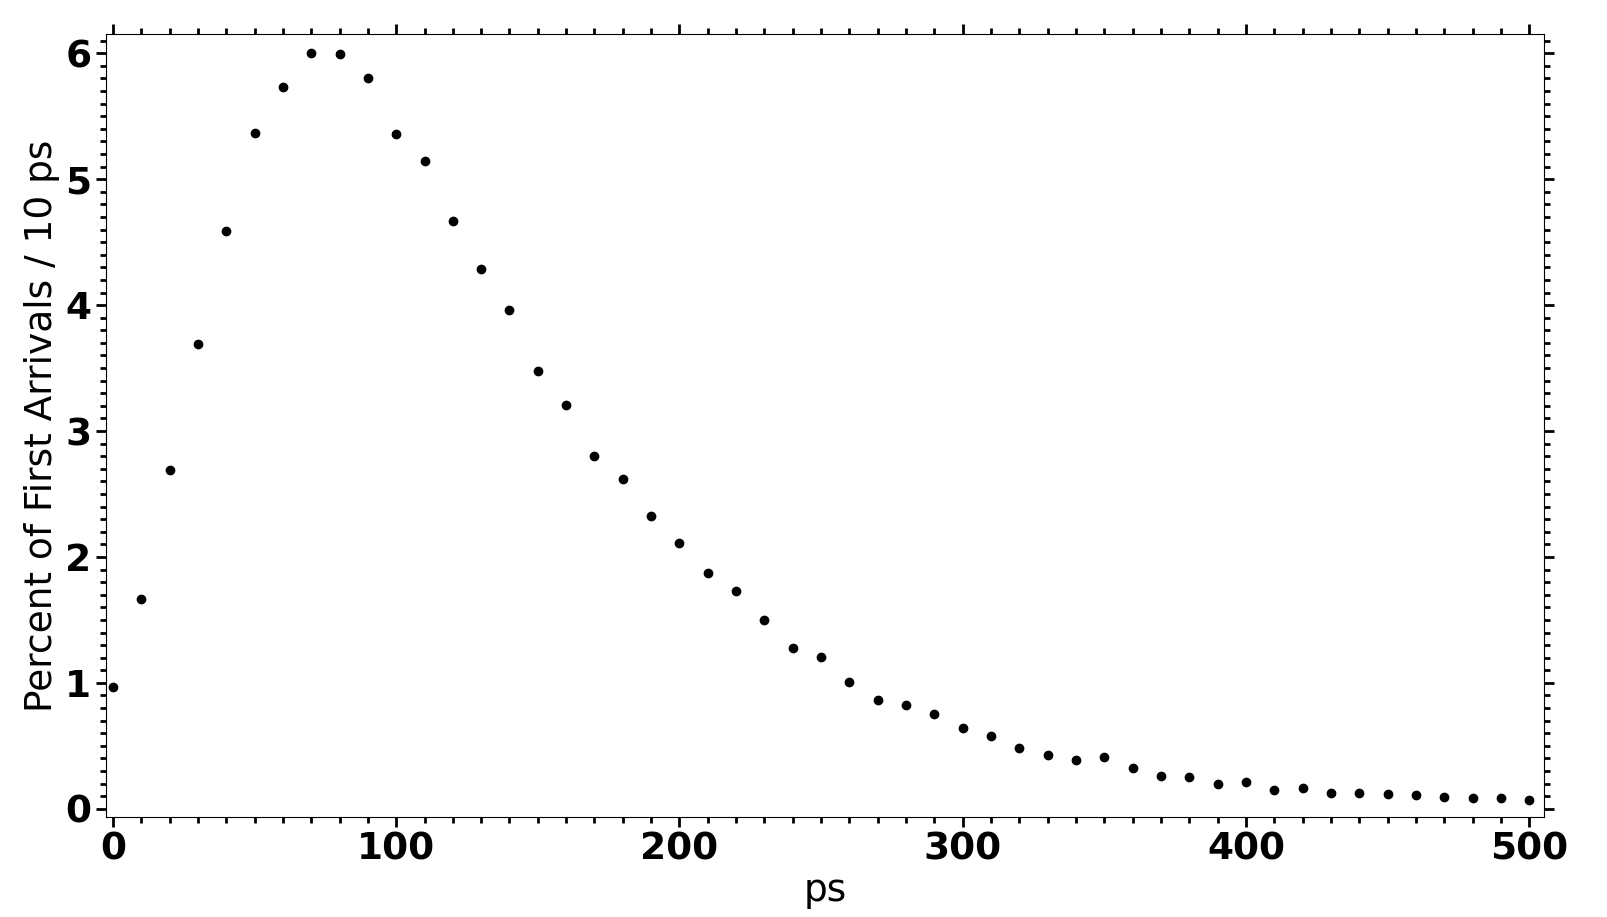
\includegraphics[angle=0,width=0.45\textwidth]{Figures/joao_tof_v1a.png}
\hfil
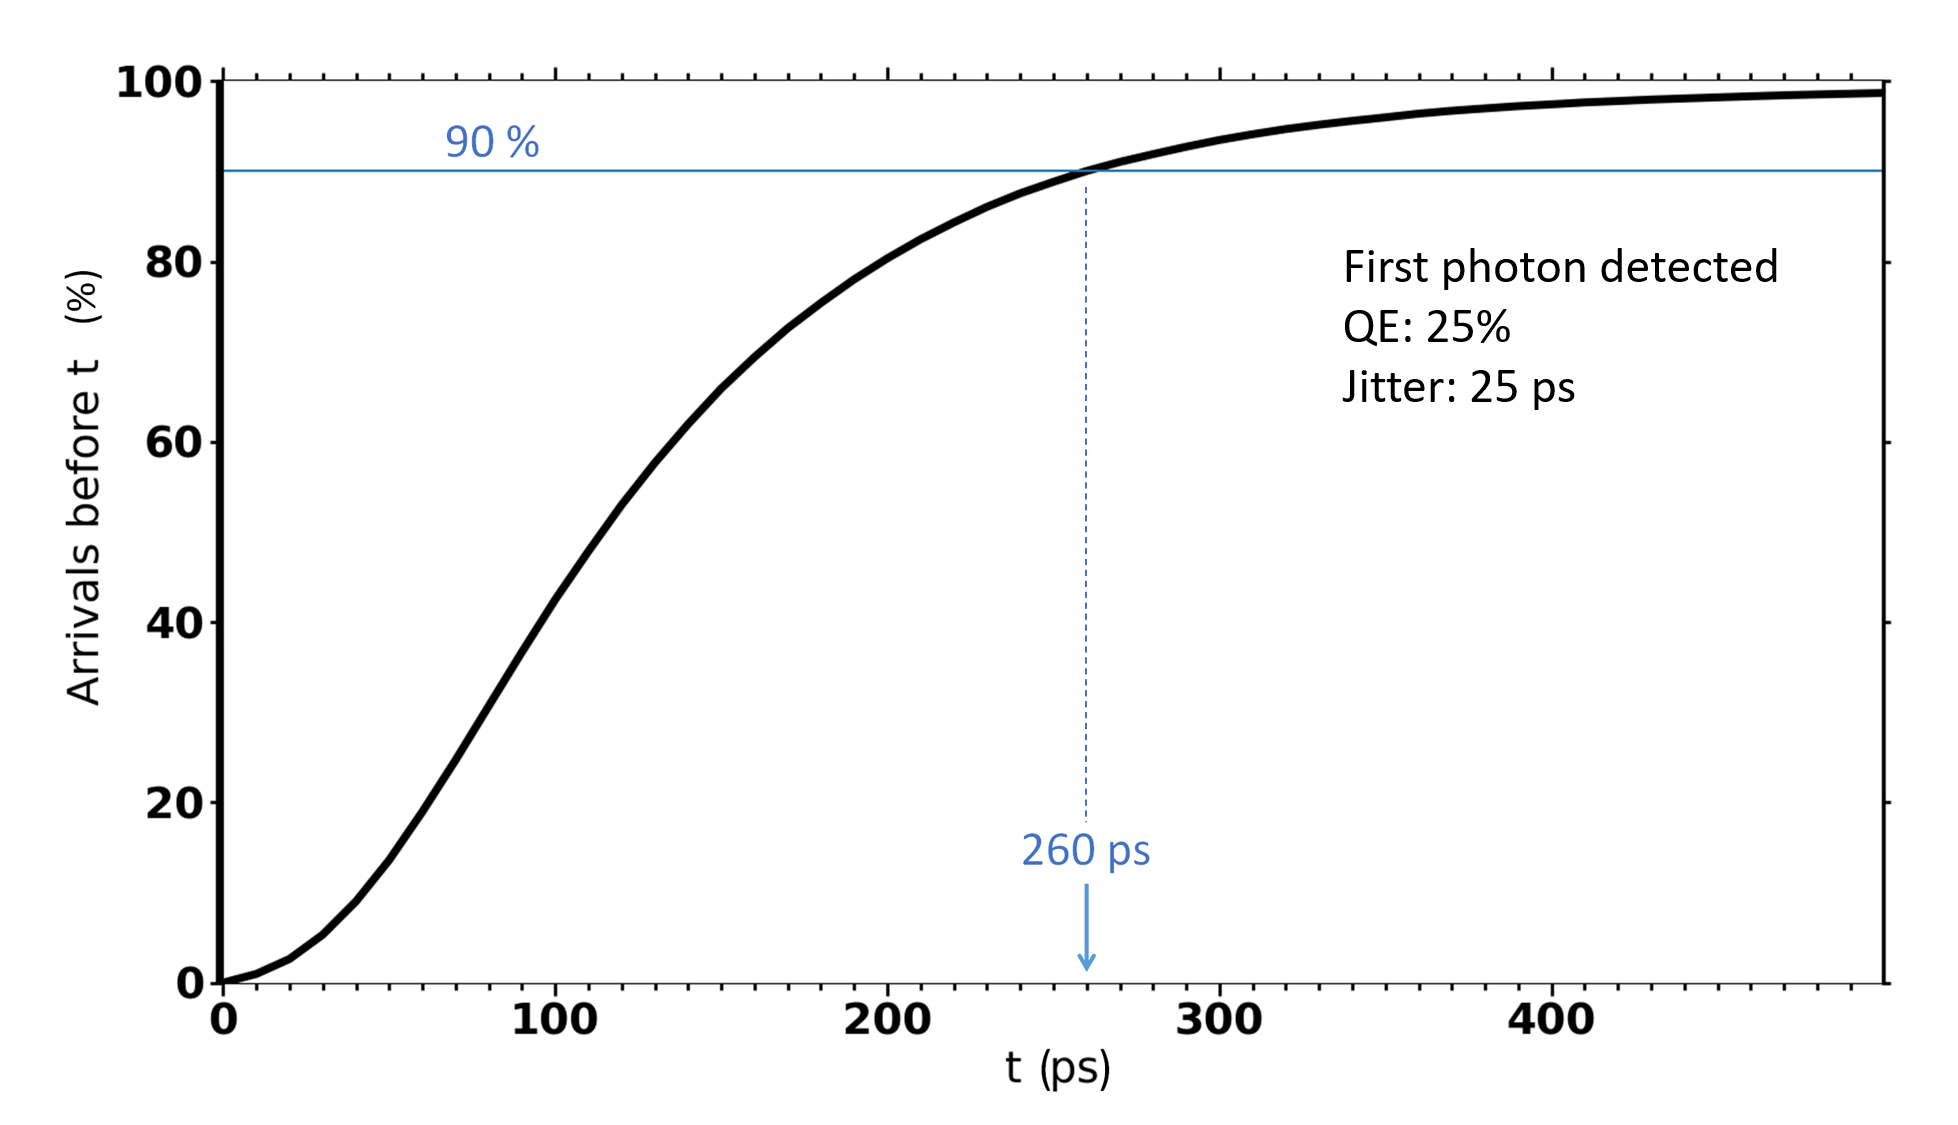
\includegraphics[angle=0,width=0.45\textwidth]{Figures/joao_TOFIntegralPlotV2a.png}
\caption{ Left: Histogram of TOF resolution from the first photon detected. Right: Integral of the TOF histogram, xxx\% of Compton electrons have a TOF resolution lower than 270 ps.}

\label{fig:TOF_differential_integral}
\end{figure}


\section{Needle Stacking, Filtering, and Feature Recognition}
\subsection{Needle Stacking}
Andy's single continuous function?
\subsection{Filtering}
Low angular frequency due to `accidental' pileup of needles
\subsection{Feature Recognition}
Brief (very) description of use of ML and AI on high-resolution images.

\section{Imaging the Derenzo and XCAT Phantoms: Signal-to-Noise at reduced dose}
\label{Imaging_phantoms}

\subsection{Zernicke fits to low-frequency background}
\label{Zernicke_fits}

\subsection{Derenzo Phantom}
\label{Derenzo_phantom}
Description and reference for Derenzo phantom goes here

%\vspace*{-1.5in}
\begin{figure}[!ht]
\centering
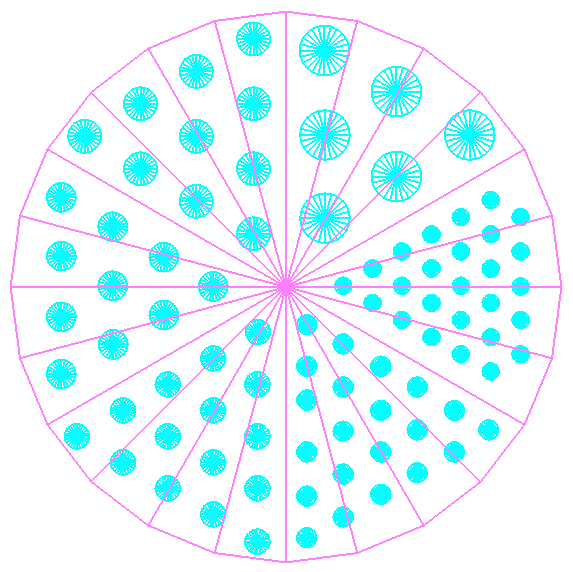
\includegraphics[angle=0,width=0.35\textwidth]{Figures/Derenzo_Truth_Focused_v1.png}
\hfil
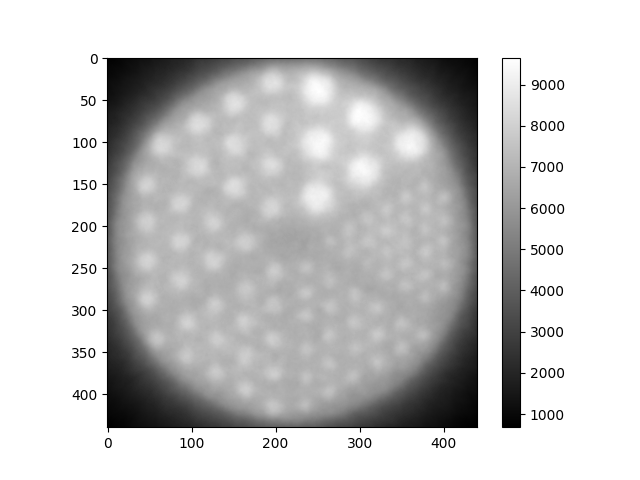
\includegraphics[width=0.5\textwidth]{Figures/Derenzo_6s_no_filter_v1.png}
\caption{Imaging the Derenzo phantom with the unfiltered back-projection of the needle stack. Left: The distribution of rods in the TOPAS model of the Derenzo phantom. The background was set to 5 MBq/kg and the rods to 15 MBq/kg. The exposure was set to 6 seconds, 1\% of 10 minutes. Right: The output of needle stacking after the simulation. The colormap corresponds to how many needles are present at each location.}
\label{fig:Derenzo_phantom_imaging}
\end{figure}

\subsubsection{Signal-to-Noise at reduced dose}
Maximum likelihood fit to Derenzo phantom\\
    Model and Free Parameters\\
    S/N results \\


\subsection{XCAT brain phantom}
\label{XCAT_brain phantom}

Hoffman brain reference (reasoning to 4:1 uptake) \\
Doses to white and grey matter, timing \\
Conversion to total positrons per cubic cm \\
Three figures: raw output, fourier filtered, fourier+zernike filtered \\

%\vspace*{-1.5in}
\begin{figure}[!ht]
\centering
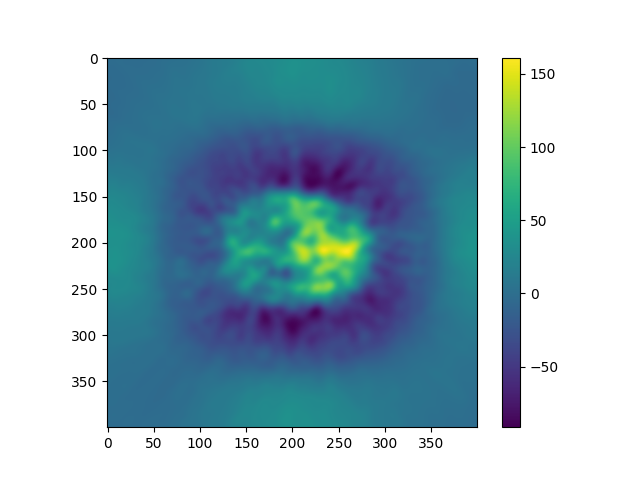
\includegraphics[angle=0,width=0.65\textwidth]{Figures/brain_1sigma.png}
\caption{Imaging the XCAT brain phantom with the unfiltered back-projection of the needle stack. Left: the projected input source distribution density of annihilations with a 10-minute exposure using xxx Bq of \F18 in the rods and xxx Bq in the surrounding volume. Middle: the reconstructed projected image from summing the weights of needles crossing each voxel.
  Right: the reconstructed projected image after subtracting a least-mean-squares fit to the first xxx terms of an expansion in Zernike functions.}
\label{fig:XCAT_brain_phantom_imaging}
\end{figure}

\subsubsection{Signal-to-Noise for the XCAT brain phantom at reduced dose}
Maximum likelihood fit to XCAT brain phantom\\
    Model and Free Parameters\\
    S/N results \\

%\subsubsection{XCAT Lung Phantom}
%PET can be used to diagnose pneumonia that does not show up well in a CT scan~\cite{Kono_pneumonia_2015}.
%\vspace*{-1.5in}
%\begin{figure}[!ht]
%\centering
%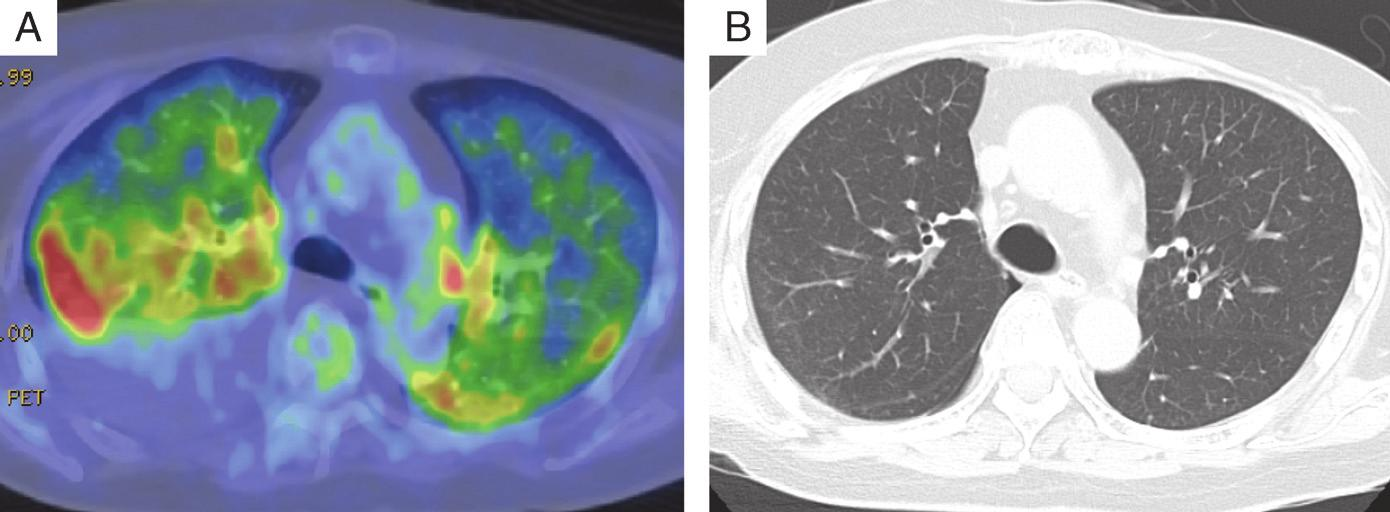
\includegraphics[angle=0,width=0.65\textwidth]{Figures/Kono_PET_Lung_2015.jpg}
%\caption{xxx Imaging the XCAT lung phantom with the unfiltered back-projection of the needle stack. Left: the projected input source distribution density of %annihilations with a 10-minute exposure using xxx Bq of \F18 in the rods and xxx Bq in the surrounding volume. Middle: the reconstructed projected image from %summing the weights of needles crossing each voxel.
%  Right: the reconstructed projected image after subtracting a least-mean-squares fit to the first xxx terms of an expansion in Zernike functions.xxx}
%\label{fig:XCAT_lung_phantom_imaging}
%\end{figure}

%\subsubsection{Signal-to-Noise for the XCAT lung phantom at reduced dose}%
%Maximum likelihood fit to XCAT brain phantom\\
%    Model and Free Parameters\\
%    S/N results \\

\clearpage
\section{Summary and Prospects}
\label{Summary}
We have used the TOPAS simulation framework to characterize the performance of a TOF-PET detector based on an ionization-sensitive low-Z persistent medium and fast MCP-based photodetectors to record the chain of Compton scatterings of the annihilation gamma rays. The time-ordering of the successive gamma scatters in the chain is time-ordered using the energies and relative positions of the scatterings. In-patient scattering is identified by measuring the component of the LOR out of the scattering planes, the correlation of the polar angles resulting from the entanglement of the two gamma polarizations, and the reconstructed gamma energies. Results are presented for the XCAT brain and  Derenzo phantoms.

The parametric simulation includes the effects of positron multiple-scattering before annihilation, localization of the first gamma interaction point at each end of the LOR, including which end is the start of the Compton recoil track,
energy resolution, TOF resolution, in-patient scattering, and mis-identification of the first cluster in the chain.

We present images of the phantoms at a dose of xxx Bq/cc in the signal region of interest and a dose of xxx Bq/cc in the background. A signal-to-noise ratio of xxx and xxx are achieved for the Derenzo and XCAT phantoms, respectively.

We have in addition simulated a detector based on photo-switchable fluors~\cite{PET_NIM_paper} using a voxelized analysis in which the Compton electron tracks are reconstructed with a simple seed-shoulder cluster algorithm to measure the ionization and direction.  A signal-to-noise ratio of xxx and xxx are achieved for the Derenzo and XCAT phantoms, respectively, lower than the ideal case by approximately xxx \%.

The prospects for the technique depend on finding or developing an appropriate persistent low-Z medium. Among candidates, photo-switchable dyes in solution with a fast scintillator and energy-transfer-enhancing mediators may be possible~\cite{Eric_CPAD}.

% Aide-memoire of figures we might want (but probably don't-- very old list)
\begin{comment}

List of other figures to consider
\section{List of Figures}
\listoffigures
%\setcounter{lofdepth}{2}% include subcaptions in listoffigures


5. TOF resolution- all correct, correct clusters one wrong end, one
wrong cluster correct ends.

6. Impact parameter resolution - all correct, correct clusters one
wrong end, one wrong cluster correct ends. (Patrick plot)

7. Impact parameter resolution - with and without in-patient scattering
(IPS).

8. In-patient scattering figure. (just refer to NIM paper?)\\

9. Energy resolution (after cluster-finding) - 1,2,5\%

10. Needle stack with energy  and TOF cuts w and wo in-patient
scattering.

\end{comment}

\section{Appendix A: Cluster Finding}
\label{Cluster_Finding}

The use of a persistent medium such as a Switchillator~\cite{PET_NIM_paper} allow multiple cycles of excitation and recording
of the fluorescence for molecules activated by recoil electron
ionization. Here we present a simulation of going beyond the ideal case above in reconstructing the time-ordered chain of scatterings to estimate the efficiencies for reconstructing the LOR.

The simulation code first voxelizes a volume of xxx by xxx
mm containing the electron track, summing the energy deposited in each
voxel (xxx- how does this work- xxx?). A clustering-algorithm links the
eight adjacent voxels with energies over a `shoulder'
threshold~\cite{Amidei_CDF_trigger_1988,PET_NIM_paper}. A higher `seed'
threshold is then applied to identify voxels to which the
nearest-neighbor algorithm is applied. The resulting list of clusters
is then curated to merge nearby clusters separated by a small number of
missing voxels xxx can we be specific somewhere else? xxx.

In the following figures, we label the ordering of the true gamma scatterings by
arabic numerals, i.e. 1, 2, ... N. The reconstructed clusters are ordered by Greek letters, with the cluster identified as being the first scatter being $\alpha$, followed by $\beta,\gamma$ etc.
A correct identification of the first true scatter being correctly ordered is thus given by the frequency of matching the $\alpha$ cluster to the N=1 scatter.

Figure~\ref{fig:cf_1st_plot} plots the fraction of correct identifications of the reconstructed $\alpha$ (squares), $\beta$  (circles); $\gamma$ (rhomboids); and $\delta$ (crosses) clusters versus the true order $N_i$, after the kinematic constraints to time-order the clusters have been applied.  The correct first scatter is identified for xxx \% of the gammas; the correct first scatter is included in the first three ($\alpha,\beta,\gamma$ reconstructed clusters xxx \%.

Figure~\ref{fig:cf_2nd_plot} shows the energy in cluster $\alpha$ versus the true energy in N$_1$,
                in $\beta$ vs in N$_2$, in $\gamma$ vs in N$_3$, in $\delta$ vs in
                N$_4$.

The energy of the recoil electron versus the scattering angle in the
                N$_1$ scatter for the true first scatter (N=1) in solid circles and the reconstructed first scatter ($\alpha$) in open circles is displayed in Figure~\ref{fig:cf_3rd_plot}.

Figure~\ref{fig:cf_4th_plot} displays the distance to the entrance window for $N_1$ (squares);
                $N_2$ (circles);$N_3$ (rhomboids) scatters (solid symbols) and for the $\alpha,\beta,\gamma$ reconstructed ordering (the corresponding open symbols).

The distance between the true point of first interaction of the gamma and the reconstructed interaction point for $\alpha$ (squares);
$\beta$ (circles);$\gamma$ (rhomboids); and $\delta $ (crosses) clusters is shown in
Figure~\ref{fig:cf_5th_plot}.  Figure~\ref{fig:cf_6th_plot} shows
   the distribution in distance between the reconstructed and true annihilation points for the Derenzo phantom.The inset shows the distribution on an expanded scale to accommodate  the broad distribution for misidentified clusters.

 \enlargethispage*{4.1in}

\begin{figure}[p]
\vskip-0.7in
  \centering
       \begin{subfigure}{0.495\textwidth}
            \centering
                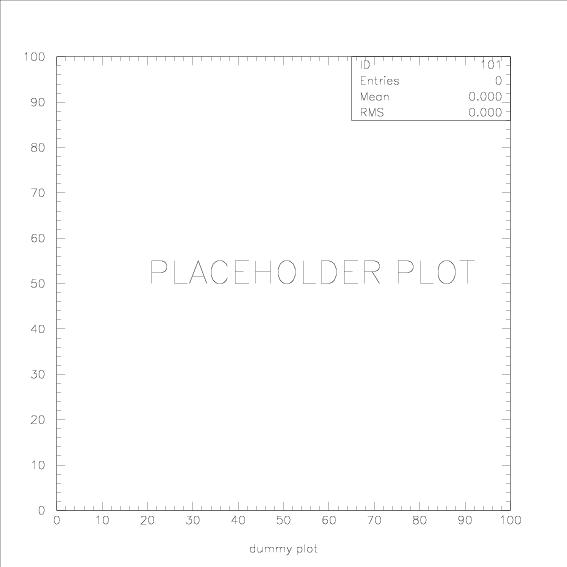
\includegraphics[width=0.6\linewidth]{Figures/dummy.jpg}
                \caption{Fraction of correct identifications of reconstructed $\alpha$ (squares), $\beta$  (circles); $\gamma$ (rhomboids); and $\delta$ (crosses) clusters vs. the true order $N_i$.}
                \label{fig:cf_1st_plot}
        \end{subfigure}
\hfil
  \begin{subfigure}{0.495\textwidth}
                \centering
                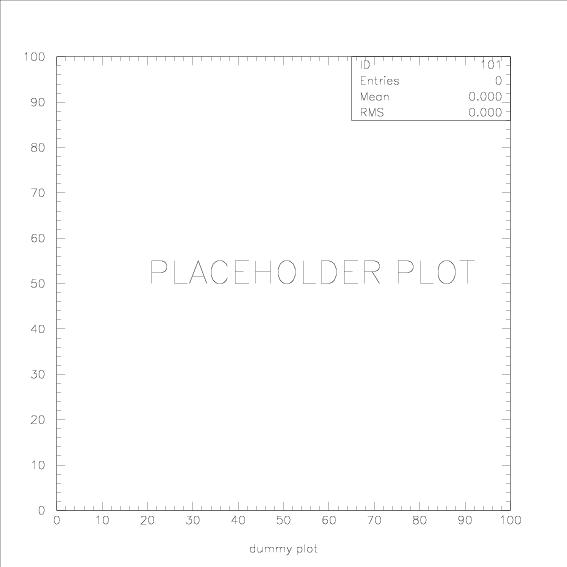
\includegraphics[width=0.6\linewidth]{Figures/dummy.jpg}
                \caption{Energy in cluster $\alpha$ vs in N$_1$,
                $\beta$ vs in N$_2$, $\gamma$ vs in N$_3$, $\delta$ vs in
                N$_4$.}
                \label{fig:cf_2nd_plot}
        \end{subfigure}


\medskip
 \begin{subfigure}{0.495\textwidth}
        \centering
                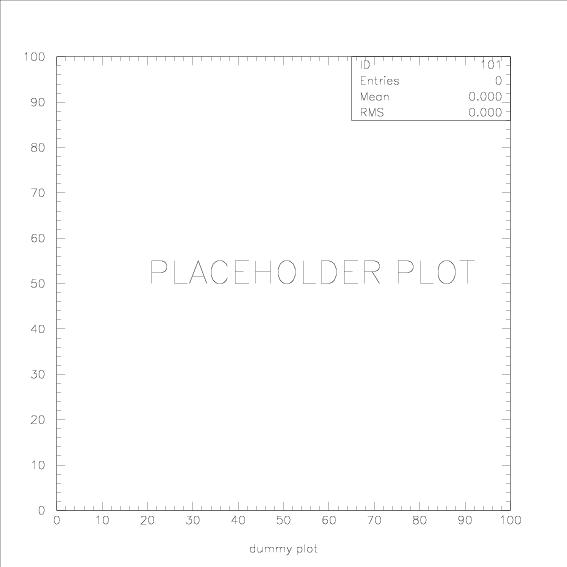
\includegraphics[width=0.6\linewidth]{Figures/dummy.jpg}
                \caption{Energy of the recoil electron versus scattering angle in the
                N$_1$ scatter for the true first scatter (N=1) (solid) and reconstructed first scatter ($\beta$) (open). }
                \label{fig:cf_3rd_plot}
        \end{subfigure}
       \hfil
        \begin{subfigure}{0.495\textwidth}
            \centering
                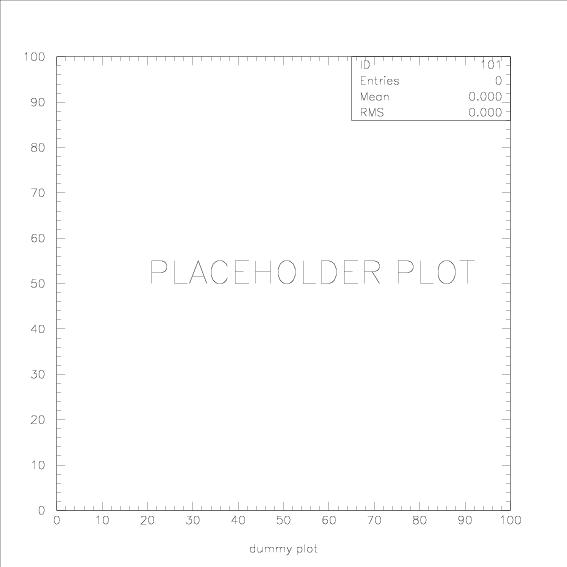
\includegraphics[width=0.6\linewidth]{Figures/dummy.jpg}
                \caption{Distance to the entrance window for $N_1$ (squares);
                $N_2$ (circles);$N_3$ (rhomboids) scatters (solid) and for the $\alpha,\beta,\gamma$ reconstructed ordering (open).}
                \label{fig:cf_4th_plot}
        \end{subfigure}
\medskip


       \begin{subfigure}{0.495\textwidth}
            \centering
                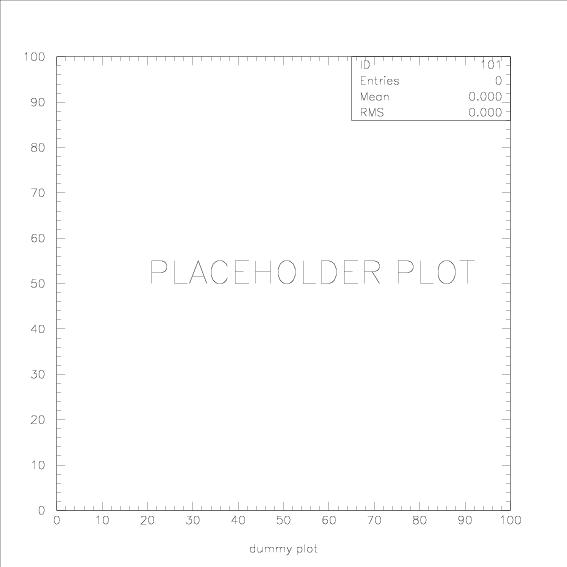
\includegraphics[width=0.6\linewidth]{Figures/dummy.jpg}
                \caption{Distance between the true first interaction point and the reconstructed point for $\alpha$ (squares);
                $\beta$ (circles);$\gamma$ (rhomboids); and $\delta $ (crosses) clusters.}
                \label{fig:cf_5th_plot}
        \end{subfigure}
        \hfil
        \begin{subfigure}{0.495\textwidth}
            \centering
                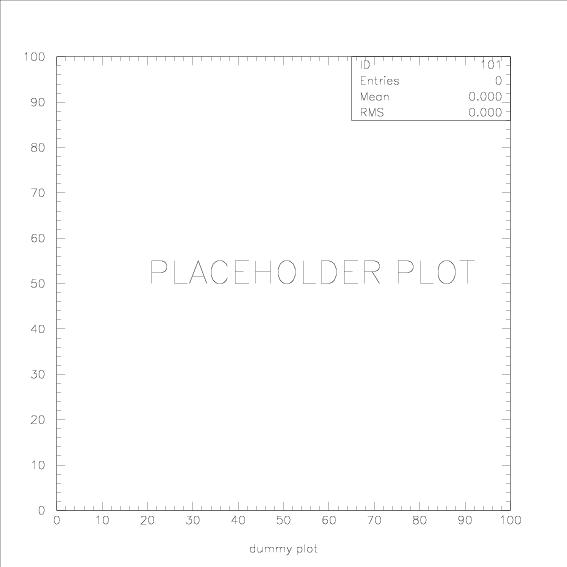
\includegraphics[width=0.6\linewidth]{Figures/dummy.jpg}
                \caption{Distribution in distance between reconstructed and true annihilation points for the Derenzo phantom. The inset shows the distribution on an expanded scale to accommodate misidentified clusters.}
                \label{fig:cf_6th_plot}
        \end{subfigure}

\caption{Comparisons of the reconstructed event after cluster finding and kinematic time-ordering with the true information from the simulation.\\
a)The fraction of correct identifications of the reconstructed $\alpha$ (squares), $\beta$  (circles); $\gamma$ (rhomboids); and $\delta$ (crosses) clusters versus the true order $N_i$.\\
b) Energy in cluster $\alpha$ vs in N$_1$, in $\beta$ vs in N$_2$, in $\gamma$ vs in N$_3$, in $\delta$ vs in N$_4$.\\
c) The energy of the recoil electron versus the scattering angle in the
                N$_1$ scatter for the true first scatter (N=1) in solid circles and the reconstructed first scatter ($\beta$) in open circles.\\
d) Distance to the entrance window for $N_1$ (squares);
                $N_2$ (circles);$N_3$ (rhomboids) scatters (solid symbols) and for the $\alpha,\beta,\gamma$ reconstructed ordering (open symbols).\\
e) Distance between the true first interaction point of the gamma and the reconstructed interaction point for $\alpha$ (squares);
                $\beta$ (circles);$\gamma$ (rhomboids); and $\delta $ (crosses) clusters.\\
f) The distribution in distance between the reconstructed and true annihilation points for the Derenzo phantom. The inset shows the distribution on an expanded scale to accommodate  the broad distribution for misidentified clusters. }
\label{fig:cluster_finding}
\end{figure}


%\vspace*{-1.5in}
\begin{figure}[!ht]
\centering
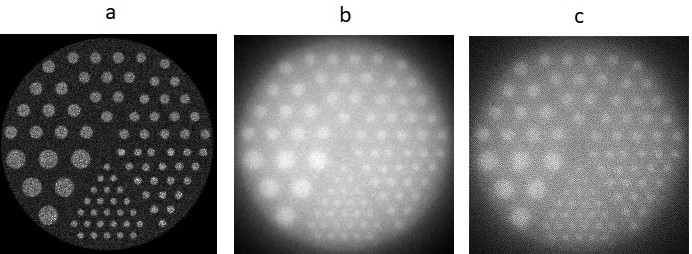
\includegraphics[angle=0,width=0.65\textwidth]{Figures/ZernikeFitDerenzoMOCK_crop_v1a.jpg}
\caption{The corresponding three images of the Derenzo phantom from the parametric simulation shown in Fig.~\ref{fig:Derenzo_phantom_imaging} but using a voxelized image and the simple seed-shoulder cluster finding algorithm~\cite{Amidei_CDF_trigger_1988,PET_NIM_paper}.}
\label{fig:CF_Derenzo_phantom_imaging}
\end{figure}


\clearpage

 \section{Acknowledgements}
Christian Buck, Michael Gross, Mary Heinz, Yifan Zhao, Paul Segars

A. Squires was supported by the Neubauer Family Foundation and the
University of Chicago Materials Research Science and Engineering
Center, which is funded by the National Science Foundation under award
number DMR-2011854. P. La Riviere was partially supported from NIH
R01EB026300. The Geant4 simulation and code development by A. Elagin
for neutrinoless double-beta decay were supported by the DOE under
contract DE-SC0008172. Materials and supplies and support for drafting
graphics were provided by the Physical Sciences Division (PSD) of the
University of Chicago. The student authors were supported by the
University's Enrico Fermi Institute, the College, and the PSD. This
work made use of the shared facilities at the University of Chicago
Materials Research Science and Engineering Center, supported by
National Science Foundation under award number DMR-2011854

% BIBLIOGRAPHY
 \begin{thebibliography}{99}
%1
\bibitem{Vandenberghe_Moskal_Karp_review_2020}
S. Vandenberghe, P. Moskal, J. S. Karp;
{\it  State of the art in total body PET}\\
 EJNMMI Phys. 2020 May 25;7(1):35.\\
doi: 10.1186/s40658-020-00290-2.

%2
\bibitem{Vaquero_Kinehan_review_2015} J. J. Vaquero and P. Kinahan; {\it Positron
  Emission Tomography: Current Challenges and Opportunities for
  Technological Advances in Clinical and Preclinical Imaging Systems}
  Annual Review of Biomedical Engineering Volume 17, 385; (2015)

%3
\bibitem{Phelps_Cherry_Dahlbom_book_2006} M. E.Phelps, S. R. Cherry, and M.
Dahlbom;\\
{\it PET: Physics,instrumentation, and scanners}; Springer New York
(2006)//doi.org/10.1007/0-387-34946-4

%4
\bibitem{Vandenberghe_Moskal_Karp_2020_Whole_Body_PET_2020}
S. Vandenberghe, P. Moskal, J.S. Karp;
{\it  State of the art in total body PET}\\
 EJNMMI Phys. 2020 May 25;7(1):35.\\
doi: 10.1186/s40658-020-00290-2. PMID: 32451783; PMCID: PMC7248164.
%note- not a duplicate of their 2015 review

%5
\bibitem{Cherry_Explorer_scattering_2019}
R. D. Badawi, H. Shi, and S. R. Cherry et al.\\
{\it First Human Imaging Studies with the EXPLORER Total-Body PET Scanner};\\
J Nucl Med. 2019 Mar; 60(3): 299-303. doi: 10.2967/jnumed.119.226498
%PMCID: PMC6424228 PMID: 30733314

%6
 \bibitem{Lee_Levin_100ps_2021}   M.S. Lee, J. Cates, A. Gonzalez-Montoro, and C. Levin;\\
  {\it High-resolution time-of-flight PET detector with 100 ps coincidence time resolution
  using a side-coupled phoswich configuration};\\
  Phys. Med. Biol. in press: https://doi.org/10.1088/1361-6560/ac01b5 (2021)

%7
\bibitem{lecoq_2019} P.~Lecoq, C.~Morel and J.~Prior,
{\it Case for setting up a 10ps challenge: A step toward reconstruction-less TOF-PET};\\
Nuovo Cim. C \textbf{43} (2020) no.1, 2 doi:10.1393/ncc/i2020-20002-y

%8
\bibitem{Credo} T. Credo, H. Frisch, H.
Sanders, R. Schroll, and F. Tang;\\
 {\it Picosecond Time-of-Flight Measurement for Colliders Using
  Cherenkov Light}\\
Proceedings of the IEEE, Rome, Italy, Oct. 2004; Nuclear Science
Symposium Conference Record, 2004 IEEE, Vol. 1.

%9
\bibitem{Ohshima} K. Inami, N. Kishimoto, Y. Enari, M. Nagamine, and T.
Ohshima; {\it  A 5-ps Tof-counter
  with an MCP-PMT}; Nucl. Instr. Meth. A560, p.303, 2006

%10
\bibitem{Anatoly_TestBeam_2010}
 A. Ronzhin et al., {\it Development of a 10 ps level time of flight
system in the Fermilab Test beam facility}; Nucl. Instr. Meth.
A623,931(2010).

%11
\bibitem{Cherry_Hamamatsu_2021} R. Ota, S. I. Kwon, E. Berg, F. Hashimoto, K. Nakajima, I.
Ogawa, Y. Tamagawa, T. Omura, T. Hasegawa, S. R. Cherry;\\
{\it Direct positron emission imaging: ultra-fast timing enables reconstruction-free imaging}\\
https://arxiv.org/ftp/arxiv/papers/2105/2105.05805.pdf

%12
\bibitem{Moses_Fundamental_Limits} W. W. Moses; {\it Fundamental Limits of
  Spatial Resolution in PET}; Nucl Instrum Methods Phys Res A. 2011 Aug
  21;648 Supplement 1:S236-S240. doi: 10.1016/j.nima.2010.11.092.
  %PMID: 21804677; PMCID: PMC3144741.

%13
\bibitem{history_paper} B. Adams et al.;
{\it A Brief Technical History of the Large-Area Picosecond
Photodetector (LAPPD) Collaboration}; arXiv:1603.01843

%14
\bibitem{timing_paper}
B.W. Adams, A. Elagin, H. Frisch, R. Obaid, E. Oberla, A. Vostrikov, R.
Wagner, J. Wang, M. Wetstein; {\it  Timing Characteristics of Large
Area Picosecond Photodetectors}; Nucl. Inst. Meth. Phys. Res. A. , Vol.
795, 1 (Sept. 2015).

%15
\bibitem{Limitations_Workshop_2011}  For a discussion of the factors that
determine time and space resolution in MCP-based detectors, see the
contributions to: {\it The Factors that Limit Time Resolution in
Photodetectors}; Workshop, Univ. of Chicago, Chicago, IL; 28-29 April
2011. See http://psec.uchicago.edu/workshops/

%16
\bibitem{Andrey_paper_1}
C. Aberle, A. Elagin, H.J. Frisch, M. Wetstein, L. Winslow;  {\it
Measuring Directionality in Double-Beta Decay and Neutrino Interactions
with Kiloton-Scale Scintillation Detectors}; JINST, Volume 9 (2014);
arXiv:1307.5813
%JINST 9 P06012 doi:10.1088/1748-0221/9/06/P06012

%17
\bibitem{PSEC4}
E. Oberla, J.-F. Genat, H. Grabas, H. Frisch, K. Nishimura, and G. Varner;\\
 {\it A 15 GSa/s, 1.5 GHz Bandwidth Waveform Digitizing ASIC};\\
 Nucl. Instr. Meth. A735, 21 Jan., 2014, 452;

%18
\bibitem{OTPC_paper} E. Oberla and H.J. Frisch; {\it Charged particle
  tracking in a water Cherenkov optical time-projection chamber};
  Nucl. Inst. Meth. Phys. Res. A814, 19 (April 2016);
  ISSN 0168-9002;  arXiv:1510.00947

\bibitem{Moskal_Organic_Scint_2012}
P.  Moskal,  T.  Bednarski,  et al.;
 {\it TOF-PET Detector Concept Based on Organic Scintillators};
 Nuclear Med Rev 2012; 15, suppl. C: C81-C84

%18
\bibitem{PET_NIM_paper} J.F. Shida, E. Spieglan, B.W. Adams, E. Angelico,
K. Domurat-Sousa, A. Elagin, H. J. Frisch,
P. La Rivi\`{e}re, A. H. Squires;\\
{\it Ionization-activated Multi-State Low-Z Detector Media}\\
arXiv e-Print: 2108.01715 (Aug 3, 2021);
Nucl. Inst. and Meth. A; Volume 1017, 21 November 2021, 165801;
https://doi.org/10.1016/j.nima.2021.165801\\
 This contains an extensive bibliography, which is consequently not included here.


%19
\bibitem{PET_patent} H. J. Frisch, E. J. Oberla, H.-J. Kim, M. Yeh;
{\it Positron-Emission Tomography Detector Systems Based On Low-Density
Liquid Scintillators And Precise Time-Resolving Photodetectors}//
  U.S. Patent 10,132,94, Filed April 8, 2016; Issued Nov. 20, 2018

%20
\bibitem{Kamland_Zen} M. Schever; {\it Status of the Jiangmen Underground Neutrino
Observatory};\\
 Ukrainian Journal of Physics, 64(7), 635; https://doi.org/10.15407/ujpe64.7.635

%21
\bibitem{cross_sections} M.J. Berger, et al.;
 Photon Cross Sections Database; cross section data for Carbon, NIST
Standard Reference Database 8; National Institute of Standards and
Technology, Gaithersburg, Md, NBSIR 87-3597 (2010);
https://dx.doi.org/10.18434/T48G6X. Also see
reference~\cite{PDG_Groom_Klein_2019}, Fig. 33.15.

%22
\bibitem{glazer_bubble_chamber} D. A. Glaser,
{\it Some Effects of Ionizing Radiation on the Formation of Bubbles in
Liquids}; Phys. Rev. 87 (4): 665 (1952)
%Bibcode:1952PhRv...87..665G. doi:10.1103/PhysRev.87.665.

%23
\bibitem{TOPAS}
 B. Faddegon, J. Ramos-Mendez, J. Schuemann, J. Shin, J. Perl, H.
 Paganetti\\
{\it The TOPAS tool for particle simulation, a Monte Carlo simulation
tool for physics, biology and clinical research}\\
European Journal of Medical Physics;  Volume 72, P114-121, April
(2020); DOI:https://doi.org/10.1016/j.ejmp.2020.03.019

\bibitem{Oberla_thesis} E. Oberla, {\it Charged Particle Tracking in a
  Water Cherenkov Optical Time Projection Chamber}, Ph.D Dissertation,
  University of Chicago, Aug. 2015

\bibitem{Philadelphia_Drifting_Light_proceedings}
 H. J. Frisch; {\it Drifting Photons on Optical Paths, Mirrors, Sub-mm
  Resolution in Four Dimensions, and Transverse/Longitudinal Phase Space:
  Exploiting Psec Time Resolution}. Proceedings of the
  5th International Conference on Micro-Pattern Gas Detectors
  (MPGD2017); 22-26 May, 2017, Philadelphia, USA; Proceedings in Science, 2018

\bibitem{Dershowitz_phantom} Harvard is proud: He kept his pants on.

\bibitem{xcat_2010_paper} Segars WP, Sturgeon G, Mendonca S, Grimes J, Tsui BM. 4D XCAT phantom for multimodality imaging research. Med Phys. 2010 Sep;37(9):4902-15. doi: 10.1118/1.3480985. PMID: 20964209; PMCID: PMC2941518.

\bibitem{icrp89} ICRP, 2002. Basic Anatomical and Physiological Data for Use in Radiological Protection Reference Values. ICRP Publication 89. Ann. ICRP 32 (3-4).

\bibitem{icrp110} ICRP, 2009. Adult Reference Computational Phantoms. ICRP Publication 110. Ann. ICRP 39 (2).

\bibitem{icrp145} ICRP, 2020. Adult mesh-type reference computational phantoms. ICRP Publication 145. Ann. ICRP 49(3).

\bibitem{icru46} Photon, Electron, Proton and Neutron Interaction Data for Body Tissues, ICRU Report 46. International Commission on Radiation Units and Measurements, Bethesda, 1992.

\bibitem{Hamamatsu_mppc_modules_kacc9019e} Hamamatsu Corporation Technical note MPPC modules, March 2021; See Hamamatsu\_mppc\_modules\_kacc9019e.pdf

\bibitem{RISC} RISC

\bibitem{Incom_production} Minot M. J., et. al. {\it Large area
  picosecond photodetector (LAPPDTM) offers fast timing for nuclear
  physics and medical imaging}, Submitted for publication in "Il Nuovo
  Cimento" January 9, 2020

\bibitem{Buck_private_comm} Christian Buck, private communication

\bibitem{Kamland-Zen} M. Schever; {\it Status of the Jiangmen Underground Neutrino
Observatory};\\
 Ukrainian Journal of Physics, 64(7), 635; https://doi.org/10.15407/ujpe64.7.635

\bibitem{Buck_MinfangYeh_metal_loaded_2016}  Christian Buck and Minfang Yeh. Metal-loaded
organic scintillators for neutrino physics; Journal of Physics G: Nuclear and Particle
Physics, 43(9):093001, 2016.

\bibitem{PDG_Groom_Klein_2019} See D. Groom and S. Klein, LBNL Particle Data
Group;\\
https://pdg.lbl.gov/2019/reviews/rpp2018-rev-passage-particles-matter.pdf

 \bibitem{Amidei_CDF_trigger_1988} D. Amidei et al.; {\it A Two-level
 Fastbus-Based Trigger System for CDF};\\
 Nucl. Instr. and Meth. A269,  51 (1988)

\bibitem{One_parameter_fit}
E Angelico, A Elagin, HJ Frisch, M Wetstein;\\
{\it Measuring the Neutrino Event Time in Liquid Argon by a
Post-Reconstruction\
 One-parameter Fit}\\
Whitepaper submitted to Snowmass2021, https://snowmass21.org/submissions/nf\\
 arXiv preprint 2004.00580 1 April, 2020

\bibitem{Eric_CPAD} E. Spieglan; {\it Using Switchable Fluorescent
  Molecules to Image Tracks and Measure Energy in Large Liquid Double
  Beta Decay Detectors}; CPAD 2019;
  https://agenda.hep.wisc.edu/event/1391/timetable/\#20191209.detailed

\bibitem{catchall_NIM_references} See the bibliography of Ref.~\cite{PET_NIM_paper}.

\bibitem{Kono_pneumonia_2015} M. Kono, H. Yamashita, K. Kubota, T. Kano, and A. Mimori\\
{\it FDG PET Imaging in Pneumocytis Pneumonia}\\
Clinical Nuclear Medicine 40, 8 Aug. 2015
%\bibitem{Tinker} Tinker
%\bibitem{Evers} Evers

\end{thebibliography}

\end{document}
